\documentclass[letterpaper,12pt]{book}
\usepackage[margin=0.75in]{geometry}
% Wait to usepackage these until they are needed.
% \usepackage{moreverb}
% \usepackage{float}
% \usepackage{subfigure}
\usepackage{graphicx}
\usepackage{wrapfig}
\usepackage{color}
% \usepackage{epstopdf}

% Again, uncomment when/if needed.
% % Define the \sourcelst command to create a floating listing of 
% % a (separate) source file.
% \newfloat{listing}{t}{lop}
% \floatname{listing}{Listing}
% \def\sourcelst#1#2{
% \begin{listing}
% \begin{tabular}{|@{\hspace{0.04\linewidth}}c@{\hspace{0.02\linewidth}}|}
% \hline \\
% \begin{minipage}{0.94\linewidth}
% \small\listinginput{1}{#1}
% \end{minipage}
% \\ \\ \hline
% \end{tabular}
% \caption{[{\tt #1}]\ \ #2}
% \label{lst:#1}
% \end{listing}
% }

\title{{\Huge The Ames Stereo Pipeline:}\\A User's Guide to the\\NASA Ames Stereo Pipeline v1.0 ALPHA}
\author{
Michael J.~Broxton\\
Ross A.~Beyer\\
Zachary Moratto\\
Mike Lundy\\
\\
Intelligent Systems Division\\
NASA Ames Research Center\\
\\
DRAFT}

\begin{document}
\maketitle

\chapter*{Credits}

This open source version of the Ames Stereo Pipeline (OSP) was
developed by the Intelligent Robotics Group (IRG), in the Intelligent
Systems Division at NASA Ames Research Center in Moffett Field, CA. It
builds on over ten years of IRG experience developing surface
reconstruction tools for terrestrial robotic field tests and planetary
exploration. \\

{\bf Lead Developer \& IRG Project Lead:}
\begin {itemize} 
\item Michael J.~Broxton (NASA/Carnegie Mellon University)\\ {\tt
  michael.broxton@nasa.gov}\\
\end{itemize}

{\bf Development Team:}
\begin{itemize}
\item Matthew Hancher (NASA)
\item Dr.~Ross Beyer (NASA/SETI Institute)
\item Zachary Moratto (Kansas State University)
\item Dr.~Ara Nefian (NASA/Carnegie Mellon University)
\item Mike Lundy (NASA/Stinger-Ghaffarian Technologies)\\
\item Vinh To (NASA/Stinger-Ghaffarian Technologies)
\end{itemize}

{\bf Contributing Developer \& Former IRG Terrain Reconstruction Lead:}
\begin{itemize}
\item Dr.\ Laurence Edwards (NASA)
\end{itemize}

A number of student interns have made significant contributions to
this project over the years: Sasha Aravkin (Washington State
University), Kyle Hussman (California Polytechnic Institute), Patrick
Mihelich (Stanford University), Melissa Bunte (Arizona State
University), Matthew Faulkner (Massachusetts Institute of Technology),
Todd Templeton (UC Berkeley), Morgon Kanter (Bard College), Kerri
Cahoy (Stanford University), and Ian Saxton (UC San Diego).

The open source stereo pipeline leverages stereo image processing
work, past and present, led by Dr. Laurence Edwards, Eric Zbinden
(formerly NASA/QSS Inc.), Dr.~Michael Sims (NASA), and others in the
Intelligent Systems Division at NASA Ames Research Center. It has
benefited substantially from the contributions of Dr.~Keith Nishihara
(formerly NASA/Stanford), Randy Sargent (NASA/Carnegie Mellon
University), Dr.~Judd Bowman (formerly NASA/QSS Inc.), Clay Kunz
(formerly NASA/QSS Inc.), and Dr.~Matthew Deans (NASA).

\section*{Acknowledgements}

The initial adaptation of Ames' stereo surface reconstruction tools to
orbital imagers was a result of a NASA funded, industry led, project
to develop automated Digital Elevation Model generation techniques for
the Mars Global Surveyor (MGS) mission. Our work with the project's
Principle Investigator, Dr.~Michael Malin of Malin Space Science
Systems (MSSS), and Co-Investigator, Dr.~Laurence Edwards of NASA
Ames, inspired the idea of making stereo surface reconstruction
technology available and accessible to a broader community.  We thank
Dr.~Malin and Dr.~Edwards for providing the initial impetus that in no
small way made this open source stereo pipeline possible, and we thank
Dr.~Michael Caplinger, Joe Fahle and others at MSSS for their help and
technical assistance.

We'd also like to thank our friends and collaborators Dr.~Randolph
Kirk, Dr.~Brent Archinal, Trent Hare, and Dr.~Mark Rosiek of the USGS
Astrogeology Branch in Flagstaff, AZ for their encouragement and
willingness to share their experience and expertise by answering many
of our technical questions.  We also thank them for their ongoing
effort to help us evaluate our work.  Thanks also to the USGS ISIS
team, especially Jeff Anderson and Kris Becker, for their help in
integrating this version of the stereo pipeline with the USGS ISIS
software package.

Thanks go also to Prof.~Mark Robinson, Jacob Danton, Ernest
Bowman-Cisneros, Dr.~Sam Laurence, and Melissa Bunte at Arizona State
University for their help in adapting the Ames' stereo pipeline to
lunar data sets including the Apollo Metric Camera.

Finally, we thank Melissa Bunte, Dr.~Ara Nefian, and Dr.~Laurence
Edwards for their contributions to this documentation, and Dr.~Terry
Fong (IRG Group Lead) for his management and support of the open
source \& public software release process.

Portions of this software were developed with support from the
following NASA funding sources: the Mars Technology Program, the Mars
Critical Data Products Initiative, the Mars Reconnaissance Orbiter
mission, the Applied Information Systems Research program grant
\#06-AISRP06-0142, the Lunar Advanced Science and Exploration Research
(LASER) program grant \#07-LASER07-0148, and the ESMD Lunar Mapping and
Modeling Program.

\tableofcontents
\chapter{Introduction}

\acresetall

The \acsu{NASA} \ac{ASP} is a suite of automated geodesy and
stereogrammetry tools designed for processing planetary imagery
captured from orbiting and landed robotic explorers on other planets
or here on earth.  It was designed to process stereo imagery captured
by \ac{NASA} and commerical spacecraft and produce cartographic
products including \acp{DEM} (digital elevation models), ortho-projected imagery, and 3D models.
These data products are suitable for science analysis, mission
planning, and public outreach.

\begin{figure}[tb]
   \centering
   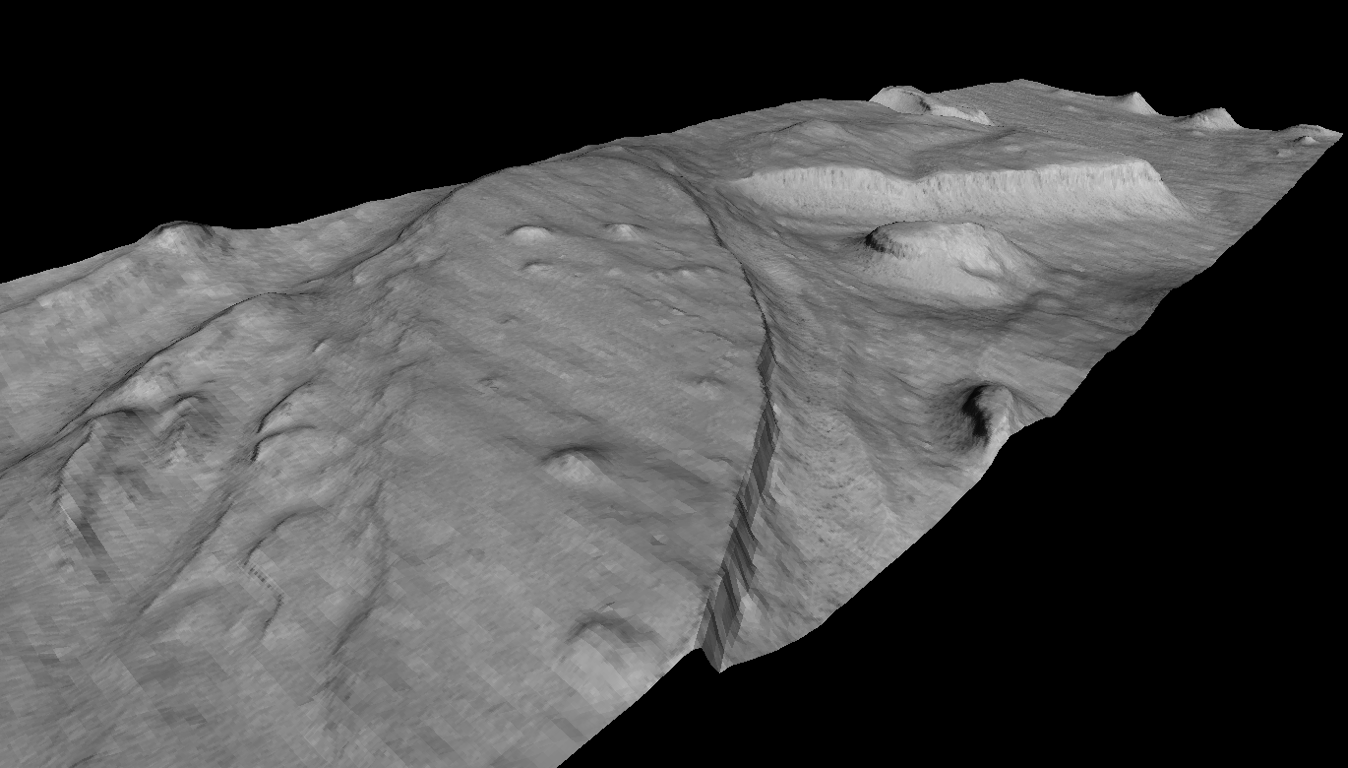
\includegraphics[width=6.5in]{images/introduction/p19view2.png}
   \caption{This 3D model was generated from a \acf{MOC} image
     pair M01/00115 and E02/01461 (34.66N, 141.29E).  The complete
     stereo reconstruction process takes approximately thirty minutes on
     a 3.0~GHz workstation for input images of this size ($1024 \times 8064$
     pixels).  This model, shown here without vertical
     exaggeration, is roughly 2~km wide in the cross-track
     dimension. }
   \label{fig:p19}
\end{figure}

\section{Background}

The \ac{IRG} at the NASA Ames Research Center has been developing
3D surface reconstruction and visualization capabilities for planetary
exploration for more than a decade.  First demonstrated during the
Mars Pathfinder Mission, the \ac{IRG} has delivered tools providing
these capabilities to the science operations teams of the Mars Polar
Lander (MPL) mission, the \ac{MER} mission, the \ac{MRO} mission,
and most recently the \ac{LRO} mission. A critical component
technology enabling this work is the \acf{ASP}.  The Stereo Pipeline
generates high quality, dense, texture-mapped 3D surface models
from stereo image pairs.

Although initially developed for ground control and scientific
visualization applications, the Stereo Pipeline has evolved in recent
years to address orbital stereogrammetry and cartographic
applications.  In particular, long-range mission planning requires
detailed knowledge of planetary topography, and high resolution
topography is often derived from stereo pairs captured from orbit.
Orbital mapping satellites are sent as precursors to planetary bodies
in advance of landers and rovers.  They return a wealth of imagery and
other data that helps mission planners and scientists identify areas
worthy of more detailed study. Topographic information often plays a
central role in this planning and analysis process.

Our recent development of the Stereo Pipeline coincides with a
period of time when \ac{NASA} orbital mapping missions are returning
orders of magnitude more data than ever before.  Data volumes from
the Mars and Lunar Reconnaissance Orbiter missions now measure in
the tens of Terabytes.  There is growing consensus that existing
processing techniques, which are still extremely human intensive
and expensive, are no longer adequate to address the data processing
needs of \ac{NASA} and the Planetary Science community.  To pick
an example of particular relevance, the \ac{HiRISE} instrument has
captured a few thousand stereo pairs.
Of these, only about a hundred stereo pairs have been processed to
date; mostly on human-operated, high-end photogrammetric workstations.
It is clear that much more value could be extracted from this
valuable raw data if a more streamlined, efficient process could be
developed.

The Stereo Pipeline was designed to address this very need.  By
applying recent advances in robotics and computer vision, we have
created an {\em automated} process that is capable of generating high
quality \acp{DEM} with minimal human intervention.  Users of the Stereo
Pipeline can expect to spend some time picking a handful of settings
when they first start processing a new type of imagery, but once this
is done the Stereo Pipeline can be used to process tens, hundreds, or
even thousands of stereo pairs without further adjustment.  With the
release of this software, we hope to encourage the adoption of this
tool chain at institutions that run and support these remote sensing
missions.  Over time, we hope to see this tool incorporated into
ground data processing systems alongside other automated image
processing pipelines.  As this tool continues to mature, we believe
that it will be capable of producing digital elevation models of
exceptional quality without any human intervention.

\section{Human vs. Computer: When to Choose Automation?}

When is it appropriate to choose automated stereo mapping over the use
of a conventional, human-operated photogrammetric workstation?  This
is a philosophical question with an answer that is likely to evolve
over the coming years as automated data processing technologies become
more robust and widely adopted.  For now, our opinion is that you
should {\em always} rely on human-guided, manual data processing
techniques for producing mission critical data products for missions
where human lives or considerable capital resources are at risk.  In
particular, maps for landing site analysis and precision landing
absolutely require the benefit of an expert human operator to
eliminate obvious errors in the \ac{DEM}; and also to guarantee that the
proper procedures have been followed to correct satellite telemetry
errors so that the data have the best possible geodetic control.

When it comes to using \acp{DEM} for scientific analysis, both techniques
have their merits.  Human-guided stereo reconstruction produces \acp{DEM}
of unparalleled quality that benefit from the intuition and experience
of an expert.  The process of building and validating these \acp{DEM} is
well established and accepted in the scientific community.

However, only a limited number of \acp{DEM} can be processed to this level
of quality.  For the rest, automated stereo processing can be used to
produce \acp{DEM} at a fraction of the cost.  The results are not
necessarily less accurate than those produced by the human operator,
but they will not benefit from the same level of scrutiny and quality
control.  As such, users of these \acp{DEM} must be able to identify
potential issues, and be on the lookout for errors that may result
from the improper use of these tools.

We recommend that all users of the Stereo Pipeline take the time to
thoroughly read this documentation and build an understanding of how
stereo reconstruction and bundle adjustment can be best used together to
produce high quality results. You are welcome to contact us if you have
any questions (section \ref{get-help}).

\section{Software Foundations}

\subsection{NASA Vision Workbench}

The Stereo Pipeline is built upon the Vision Workbench software
which is a general purpose image processing and computer vision
library also developed by the \ac{IRG}.  Some of the tools discussed
in this document are actually Vision Workbench programs, but any
distribution of the Stereo Pipeline requires the Vision Workbench.
Unless you're compiling the Vision Workbench and Stereo Pipeline from
source, the distinctions probably won't matter to you.


\subsection{The USGS Integrated Software for Imagers and Spectrometers}

For processing non-terrestrial NASA satellite imagery, Stereo Pipeline
must be installed alongside a copy of \ac{USGS} \ac{ISIS}. \ac{ISIS} is
however not required for processing Digital Globe images of Earth, as
described in section \ref{quickstartDG}.

\ac{ISIS} is widely used in the planetary science community
for processing raw spacecraft imagery into high level data products of
scientific interest such as map-projected and mosaicked imagery
\cite{2004LPI....35.2039A, 1997LPI....28..387G, ISIS_website}.  We
chose \ac{ISIS} because (1) it is widely adopted by the planetary
science community, (2) it contains the authoritative collection of
geometric camera models for planetary remote sensing instruments, and
(3) it is open source software that is easy to leverage.

By installing the Stereo Pipeline, you will be adding an advanced
stereo image processing capability that can be used in your existing
\ac{ISIS} workflow.  The Stereo Pipeline supports the \ac{ISIS}
``cube'' (\texttt{.cub}) file format, and can make use of the \ac{ISIS}
camera models and ancillary information (i.e. SPICE kernels) for
imagers on many \ac{NASA} spacecraft.  The use of this single standardized
set of camera models ensures consistency between products generated
in the Stereo Pipeline and those generated by \ac{ISIS}.  Also by
leveraging \ac{ISIS} camera models, the Stereo Pipeline can process
stereo pairs captured by just about any \ac{NASA} mission.


%% It might be good to add a section on terminology someday...
%\section{Terminology}
%
%DISPARTY
%
%TRIANGULATION
%
%CORRELATION
%
%BUNDLE ADJUSTMENT

\pagebreak
\section{Getting Help}\label{get-help}

All bugs, feature requests, and general discussion should be sent to
the Ames Stereo Pipeline user mailing list:
\begin{quote}
\indent \href{mailto:stereo-pipeline@lists.nasa.gov}{stereo-pipeline@lists.nasa.gov}
\end{quote}
To subscribe to this list, send an empty email message with the
subject `subscribe' (without the quotes) to:
\begin{quote}
\indent \href{mailto:stereo-pipeline-request@lists.nasa.gov}{stereo-pipeline-request@lists.nasa.gov}
\end{quote}
To contact the lead developers and project manager directly, send mail
to:
\begin{quote}
\indent \href{mailto:stereo-pipeline-owner@lists.nasa.gov}{stereo-pipeline-owner@lists.nasa.gov}
\end{quote}

\section{How to File Bug Reports} 

If Stereo Pipeline crashes or produces incorrect results, we would very
much like to hear from you. You can send an email to
\texttt{stereo-pipeline-owner@lists.nasa.gov} describing the problem. It
will be helpful to attach the logs output by \texttt{stereo} and other
tools (section \ref{logging}). In some cases we may request your input
data as well.

\section{Typographical Conventions}

Names of programs that are meant to be run on the command line are
written in a constant-width font, like the \texttt{stereo} program,
as are options to those programs.

An indented line of constant-width text can be typed into your
terminal, these lines will either begin with a `\texttt{>}' to
denote a regular shell, or with `\texttt{ISIS}' which denotes an
\ac{ISIS}-enabled shell (which means you have to set the \texttt{ISISROOT}
environment variable and sourced the appropriate \ac{ISIS} 3 Startup
script, as detailed in the \ac{ISIS} 3 instructions).
\begin{verbatim}
  > ls

  ISIS 3> pds2isis
\end{verbatim}

Italicized constant-width text denotes an option or argument that
a user will need to supply.  For example, `\texttt{stereo E0201461.map.cub
M0100115.map.cub out}' is specific, but `\texttt{stereo \textit{left-image
right-image} out}' indicates that \texttt{\textit{left-image}} and
\texttt{\textit{right-image}} are not the names of specific files,
but dummy parameters which need to be replaced with actual file
names.

Square brackets denote optional options or values to a command, and
items separated by a vertical bar are either aliases for each other, or
different, specific options.  Default arguments are prefixed by an equals
sign within parentheses, and line continuation with a backslash:

\texttt{  point2dem [-\/-help|-h] [-r moon|mars] [-s \textit{float(=0)}] $\backslash$ } \\
\hspace*{6em}\texttt{[-o \textit{output-filename}] \textit{pointcloud}-PC.tif}

The above indicates a run of the \texttt{point2dem} program.  The
only argument that it requires is a point cloud file, which is
produced by the \texttt{stereo} program and ends in \texttt{-PC.tif},
although its prefix could be anything (hence the italics for that
part).  Everything else is in square brackets indicating that they
are optional.

Both \texttt{-\/-help} and \texttt{-h} are really the same thing (both
will get you help).  Similarly, the argument to the \texttt{-r}
option must be either \texttt{moon} or \texttt{mars}.  The \texttt{-s}
option takes a floating point value as its argument, and has a
default value of zero.  The \texttt{-o} option takes a filename
that will be used as the output \ac{DEM}.

Although there are two lines of constant-width text, the backslash at the end
of the first line indicates that the command continues on the second line.  You
can either type everything into one long line on your own terminal, or use the
backslash character (or appropriate line continuation character) and a return to
continue typing on a second line in your terminal.


\section{Referencing the Ames Stereo Pipeline in Your Work}

Although no peer-reviewed paper or report yet exists which details the
Ames Stereo Pipeline (see the warning below about this being {\bf
  research} software), if you do use this software in your work, we'd
appreciate it if you referenced one or more of these abstracts:

\begin{description}
\item Moratto, Z. M., M. J. Broxton, R. A. Beyer, M. Lundy, and K. Husmann.
2010. Ames Stereo Pipeline, NASA's Open Source Automated Stereogrammetry
Software. \textit{Lunar and Planetary Science Conference} \textbf{41},
abstract \#2364.
\href{http://adsabs.harvard.edu/abs/2010LPI....41.2364M}{[ADS Abstract]}.

\item Broxton, M. J. and L. J. Edwards. 2008. The Ames Stereo Pipeline:
Automated 3D Surface Reconstruction from Orbital Imagery. \textit{Lunar
and Planetary Science Conference} \textbf{39}, abstract \#2419.
\href{http://adsabs.harvard.edu/abs/2008LPI....39.2419B}{[ADS Abstract]}.
\end{description}

\section{Warnings to Users of the Ames Stereo Pipeline}

Ames Stereo Pipeline is a {\bf research} product. There may be bugs or
incomplete features. We reserve the ability to change the API and
command line options of the tools we provide. Although we hope you will
find this release helpful, you may use it at your own risk. Please check
each release's {\bf NEWS} file to see a summary of our recent changes.

While we are confident that the algorithms used by this software are
robust, they have not been systematically tested or rigorously
compared to other methods in the peer-reviewed literature. We have a
number of efforts underway to carefully compare Stereo
Pipeline-generated data products to those produced using established
processes, and we will publish those results as they become available.
In the meantime, we {\it strongly recommend} that you consult us first
before publishing any results based on the cartographic products
produced by this software.

\chapter{Installation}

\section{Binary Installation}

This is the recommended method. Only two things are required:

\begin{description}
\item [{Stereo~Pipeline~tarball.}] The main Stereo Pipeline page is \url{http://ti.arc.nasa.gov/stereopipeline}.
In the upper-right, there is a list of files. Download the \emph{Binary}
option that matches the platform you wish to use. The required \ac{ISIS}
version is listed next to the name; choose the newest version you
have available.

\item [{\ac{USGS}~\ac{ISIS}~Binary~Distribution.}] The Stereo Pipeline depends
on \ac{ISIS} version 3 from the USGS\@. Their installation guide is at \url{http://isis.astrogeology.usgs.gov/documents/InstallGuide}.
You must use their binaries as-is; if you need to recompile, you must
follow the \emph{Source Installation} guide in Section~\ref{sec:Source-Installation}.
Note also that the \ac{USGS} does not provide any version of \ac{ISIS} but the
current one. If you need a past version, you must retain it yourself.
\end{description}

\subsection{Quickstart}
\begin{description}

\item[{Fetch~Stereo~Pipeline}] ~\\
Download the Stereo Pipeline from \url{http://ti.arc.nasa.gov/stereopipeline}.

\item [{Fetch~\ac{ISIS}\_Binaries}] ~\\
\verb#rsync -azv --delete isisdist.wr.usgs.gov::isis3_ARCH_OS/isis .#

\item [{Fetch~\ac{ISIS}\_Data}] ~\\
\verb#rsync -azv --delete isisdist.wr.usgs.gov::isis3data/data .#

\item [{Untar~\acl{ASP}}] ~\\
\verb#tar xzvf StereoPipeline-VERSION-ARCH-OS.tar.gz#

% Verbatim has way too much white space. Couldn't seem to take care of it with
% vskip/vspace negative. Sigh.
\item [{Add~Stereo~Pipeline~to~Path~(optional)}] ~\\
\verb#(bash) export PATH="/path/to/StereoPipeline/bin:${PATH}"# \\
\verb#(csh)  setenv PATH "/path/to/StereoPipeline/bin:${PATH}"#

% Grrrr. Why doesn't it keep this together? Sprinkling in \nopagebreak
% doesn't seem to work... Forcing a pagebreak instead
\pagebreak
\item[Set~Up~Isis] ~\\
\verb#(bash)# \\
\verb#    export ISISROOT=/path/to/isisroot# \\
\verb#    source $ISISROOT/scripts/isis3Startup.sh# \\
\verb#(csh)# \\
\verb#    setenv ISISROOT /path/to/isisroot# \\
\verb#    source $ISISROOT/scripts/isis3Startup.csh#

\item [{Try~It~Out!}] ~\\
See the next chapter (Chapter~\ref{ch:tutorial}) for an example!
\end{description}

\subsection{Common Traps}

Here are some errors you might see, and what it could mean. Treat
these as templates for problems--- in practice, the error messages might
be slightly different.

\begin{verbatim}
stereo: error while loading shared libraries: libisis3.so:
    cannot open shared object file: No such file or directory
\end{verbatim}

You just need to set up your ISIS environment.

\begin{verbatim}
dyld: Library not loaded: $ISISROOT/lib/libisis3.dylib
Referenced from: /some/path/goes/here/bin/program
Reason: image not found Trace/BPT trap
\end{verbatim}

You just need to set up your ISIS environment.

\begin{verbatim}
point2mesh E0201461-M0100115-PC.tif E0201461-M0100115-L.tif
[...]
99%  Vertices:   [************************************************************] Complete!
       > size: 82212 vertices
Drawing Triangle Strips
Attaching Texture Data
zsh: bus error  point2mesh E0201461-M0100115-PC.tif E0201461-M0100115-L.tif
\end{verbatim}

The source of this problem is an old version of OpenSceneGraph in
your library path. Check your \verb#LD_LIBRARY_PATH# (for Linux),
\verb#DYLD_LIBRARY_PATH# (for OSX), or your \verb#DYLD_FALLBACK_LIBRARY_PATH#
(for OSX) to see if you have an old version listed, and remove if
from the path if that is the case. It is not necessary to remove the
old versions from your computer, you just need to remove the reference
to them from your library path.

\section{\label{sec:Source-Installation}Source Installation}

This method is for advanced users only.

\subsection{Dependency List}

This is a list of direct dependencies of Stereo Pipeline. Some libraries
(like ISIS) have dependencies of their own which are not covered here.

\begin{description}
\item [{Boost}] (Required) \url{http://www.boost.org/}\\
Version 1.35 or greater is required. Along with the base library
set, the Stereo Pipeline specifically requires: Program Options, Filesystem,
Thread, and Graph.

\item [{LAPACK}] (Required)\\
There are many sources for LAPACK\@. For OSX, you can use the
vecLib framework. For Linux, you can use the netlib LAPACK/CLAPACK
distributions, or Intel's MKL, or any of a number of others. The math
is unfortunately not a hotspot in the code, though, so using a faster
LAPACK implementation will not change much. Therefore, you should
probably just use the LAPACK your package manager (RPM for Red Hat
Linux, Yast for SuSE, etc.) has available.

\item [{ISIS}] (Recommended) \url{http://isis.astrogeology.usgs.gov/documents/InstallGuide}\\
The USGS Integrated Software for Imagers and Spectrometers (ISIS) library. This
library handles the camera models and image formats used for instruments.

\item [{OpenSceneGraph}] (Optional) \url{http://www.openscenegraph.org/}\\
OpenSceneGraph is required to run the \texttt{point2mesh} tool
(See Section~\ref{point2mesh}).

\item [{Vision~Workbench}] (Required) \url{http://ti.arc.nasa.gov/visionworkbench/}\\
Vision Workbench forms much of the core processing code of the
Stereo Pipeline.

\end{description}

\subsection{Build System}

The build system is built on GNU autotools. In-depth information on
autotools is available from \url{http://sources.redhat.com/autobook/}.
The basics, however, are simple. To compile the source code, first
run \verb#./configure# from the top-level directory. This will search
for the dependencies and enable the modules you requested. There are
a number of options that can be passed to \verb#configure#; many
of these options can also be placed into a \verb#config.options#
file (in the form of \verb#VARIABLE="VALUE"#) in the same directory
as \verb#configure#. Table \ref{tab:Supported-configure-options}
lists the supported options.

\begin{table}
\begin{longtable}{|l|l|c|m{5cm}|}
\hline
\textbf{Variable Name}                & \textbf{Configure option}               & \textbf{Default} & \textbf{Function}\tabularnewline
\hline
\hline
\small\verb#PREFIX#                   & \small\verb#--prefix#                   & /usr/local       & Set the install prefix (ex: binaries will go in \$PREFIX/bin)\tabularnewline
\hline
\small\verb#HAVE_PKG_XXX#             & \small\verb#--with-xxx#                 & auto             & Set to {}``no'' to disable package XXX, or a path to only search that path\tabularnewline
\hline
\small\verb#PKG_PATHS#                & \small\verb#--with-pkg-paths#           & many             & Prepend to default list of search paths\tabularnewline
\hline
\small\verb#ENABLE_PKG_PATHS_DEFAULT# & \small\verb#--enable-pkg-paths-default# & yes              & Append built-in list of search paths\tabularnewline
\hline
\small\verb#ENABLE_OPTIMIZE#          & \small\verb#--enable-optimize#          & 3                & Level of compiler optimization?\tabularnewline
\hline
\small\verb#ENABLE_DEBUG#             & \small\verb#--enable-debug#             & no               & How much debug information?\tabularnewline
\hline
\small\verb#ENABLE_CCACHE#            & \small\verb#--enable-ccache#            & no               & Use \verb#ccache# if available\tabularnewline
\hline
\small\verb#ENABLE_RPATH#             & \small\verb#--enable-rpath#             & no               & Set RPATH on built binaries and libraries\tabularnewline
\hline
\small\verb#ENABLE_ARCH_LIBS#         & \small\verb#--enable-arch-libs#         & no               & Pass in 64 or 32 to look for libraries by default in \verb#lib64# or \verb#lib32#\tabularnewline
\hline
\small\verb#ENABLE_PROFILE#           & \small\verb#--enable-profile#           & no               & Use function profiling?\tabularnewline
\hline
\small\verb#PKG_XXX_CPPFLAGS#         &                                         &                  & Append value to CPPFLAGS for package XXX\tabularnewline
\hline
\small\verb#PKG_XXX_LDFLAGS#          &                                         &                  & Prepend value to LDFLAGS for package XXX\tabularnewline
\hline
\small\verb#PKG_XXX_LIBS#             &                                         &                  & Override the required libraries for package XXX\tabularnewline
\hline
\small\verb#PKG_XXX_MORE_LIBS#        &                                         &                  & Append to required libraries for package XXX\tabularnewline
\hline
\small\verb#ENABLE_EXCEPTIONS#        & \small\verb#--enable-exceptions#        & yes              & Use C++ exceptions? Disable at own risk.\tabularnewline
\hline
\small\verb#ENABLE_MULTI_ARCH#        & \small\verb#--enable-multi-arch#        & no               & OSX Only: Build \emph{Fat} binary with space-separated list of arches\tabularnewline
\hline
\small\verb#ENABLE_AS_NEEDED#         & \small\verb#--enable-as-needed#         & no               & Pass --as-needed to GNU linker. Use at your own risk.\tabularnewline
\hline
\end{longtable}\caption{\label{tab:Supported-configure-options}Supported configure options}
\end{table}

\end{document}

\chapter{Getting Started}


\section{Overview}

The programs in the Stereo Pipeline are command-line programs which
take a pair of images, and attempt to create a three-dimensional
point cloud from correlating them.  Then there are a few programs
that can convert that point cloud into a mesh for viewing or a
gridded terrain model for use in other ways.

So at the highest, most abstract level, if you have two image files
(say \texttt{image\_file1} and \texttt{image\_file2} ) this command
makes point clouds (and a bunch of other files):

\begin{verbatim}
    stereo image_file1 image_file2 stereo-output
\end{verbatim}
\noindent
Then you can make a mesh or a DEM file with either of the following
commands.  The \texttt{stereo-output-PC.tif} and
\texttt{stereo-output-L.tif} files are created by the \texttt{stereo}
program run above):

\begin{verbatim}
    point2mesh stereo-output-PC.tif stereo-output-L.tif

    point2dem stereo-output-PC.tif stereo-output-L.tif
\end{verbatim}
\noindent
There are a number of ways to fine-tune parameters and
analyze the results, but ultimately this software suite takes images
and builds models in a mostly automatic way.


\section{Selecting images to process}

When choosing image pairs to process, images that are taken with
similar viewing angles, lighting conditions, and significant surface
coverage overlap ($\sim80$\% is ideal) are the best suited for
creating terrain models from. Depending on the characteristics of
the mission data set and the individual images, the degree of
acceptable variation will differ. Significant differences between
image characteristics increases the error propagated through to the
resulting data products.

Images do not need to be map projected before running the \texttt{stereo}
program. That being said, for images which contain large topographic
variation (and therefore large disparity differences across the
scene--think Valles Marineris), sometimes map-projecting the images
can help, as it sometimes improves the correlation (at least until
we get our adaptive correlation window strategies in place).  However,
be careful about map-projecting.  For example, the HiRISE RDR
products, which are map projected, have been map-projected onto a
smoothed MOLA terrain model, so these images are not suitable for
stereo processing, because the act of projecting them on to a terrain
model introduces disparity into the source images that will lead
to poor results.

The images should be photometrically calibrated (in whatever fashion
suits your purposes), as excessively noisy images will not correlate
well.  If there are photometric problems with the images, those
photometric defects could be misinterpreted as topography.

The Stereo Pipeline can deal with arbitrary images with accompanying
camera information, but doing so requires a significant amount of
extra work and setup which are not covered in this document, and
are considered `advanced usage.'  The image type that is easiest
for the user to provide and for the Stereo Pipeline's \texttt{stereo}
program to ingest are ISIS 3 cube files (\texttt{.cub}).  In order
for \texttt{stereo} to utilize the detailed camera data available
for planetary data (SPICE), the images must have had ISIS's
\texttt{spiceinit} program run on them.


\section{Example data set}

The data set that is used in the tutorial and examples below is a
pair of Mars Orbiter Camera (MOC)
\citep{1992JGR....97.7699M,2001JGR...10623429M} images whose Planetary
Data System (PDS) Product IDs are M01/00115 and E02/01461.
These data can be downloaded from the PDS directly, or they can be found in
the \texttt{data/MOC/} directory of your Stere Pipeline distribution.

These raw PDS images (\texttt{M0100115.imq} and \texttt{E0201461.imq})
need to be brought in to the ISIS environment and radiometrically
calibrated.  Fortunately, ISIS has a simple command for that.  You
will need to be in an ISIS environment (have set the \texttt{ISISROOT}
environment variable and sourced the appropriate ISIS 3 Startup
script, as detailed in the ISIS 3 instructions, we will denote this
state with the `\texttt{ISIS 3>}' prompt).  Then you can use the
\texttt{mocproc} program.

\begin{verbatim}
    ISIS 3> mocproc from= M0100115.imq to= M0100115.cub Mapping= NO
\end{verbatim}
\noindent
There are also \texttt{Ingestion} and \texttt{Calibration} parameters
whose defaults are `\texttt{YES}' which will bring the image into
the ISIS format and perform radiometric calibration.  By setting
the \texttt{Mapping} parameter to `\texttt{NO}' the resultant file
will be an ISIS cube file that is calibrated, but not map-projected.
Note that while we have not explicitly run \texttt{spiceinit}, the
Ingestion portion of \texttt{mocproc} quietly ran \texttt{spiceinit}
for you (you'll find the record of it in the ISIS Session Log,
usually written out to a file named \texttt{print.prt}).

\begin{figure}[b!]
\begin{minipage}{5.2in}
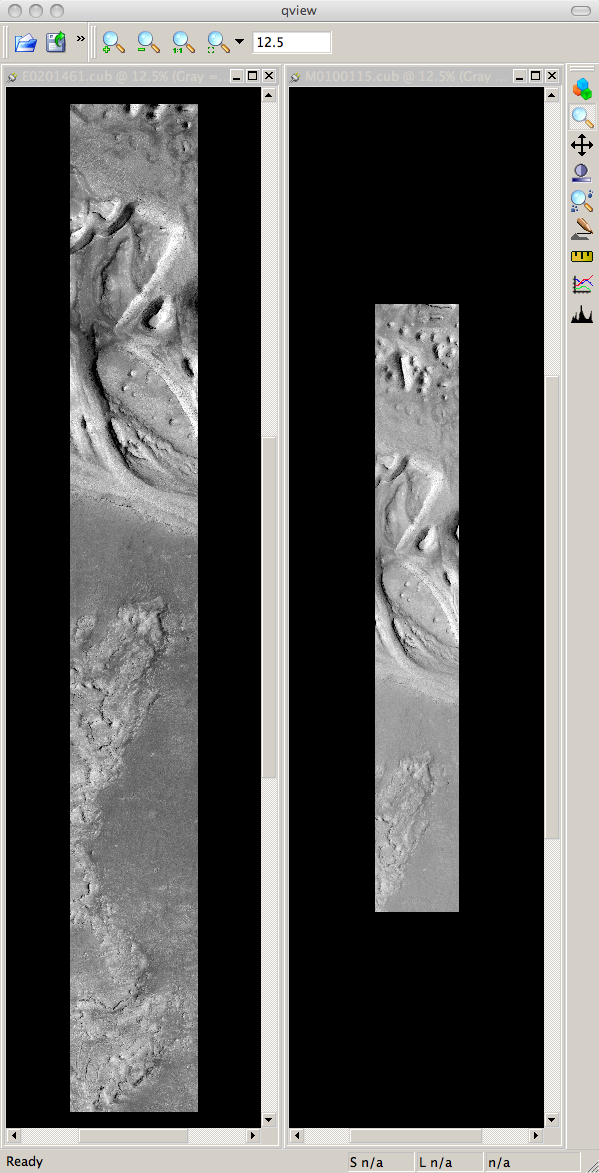
\includegraphics[height=3.7in]{images/p19-images.png}
\hfill
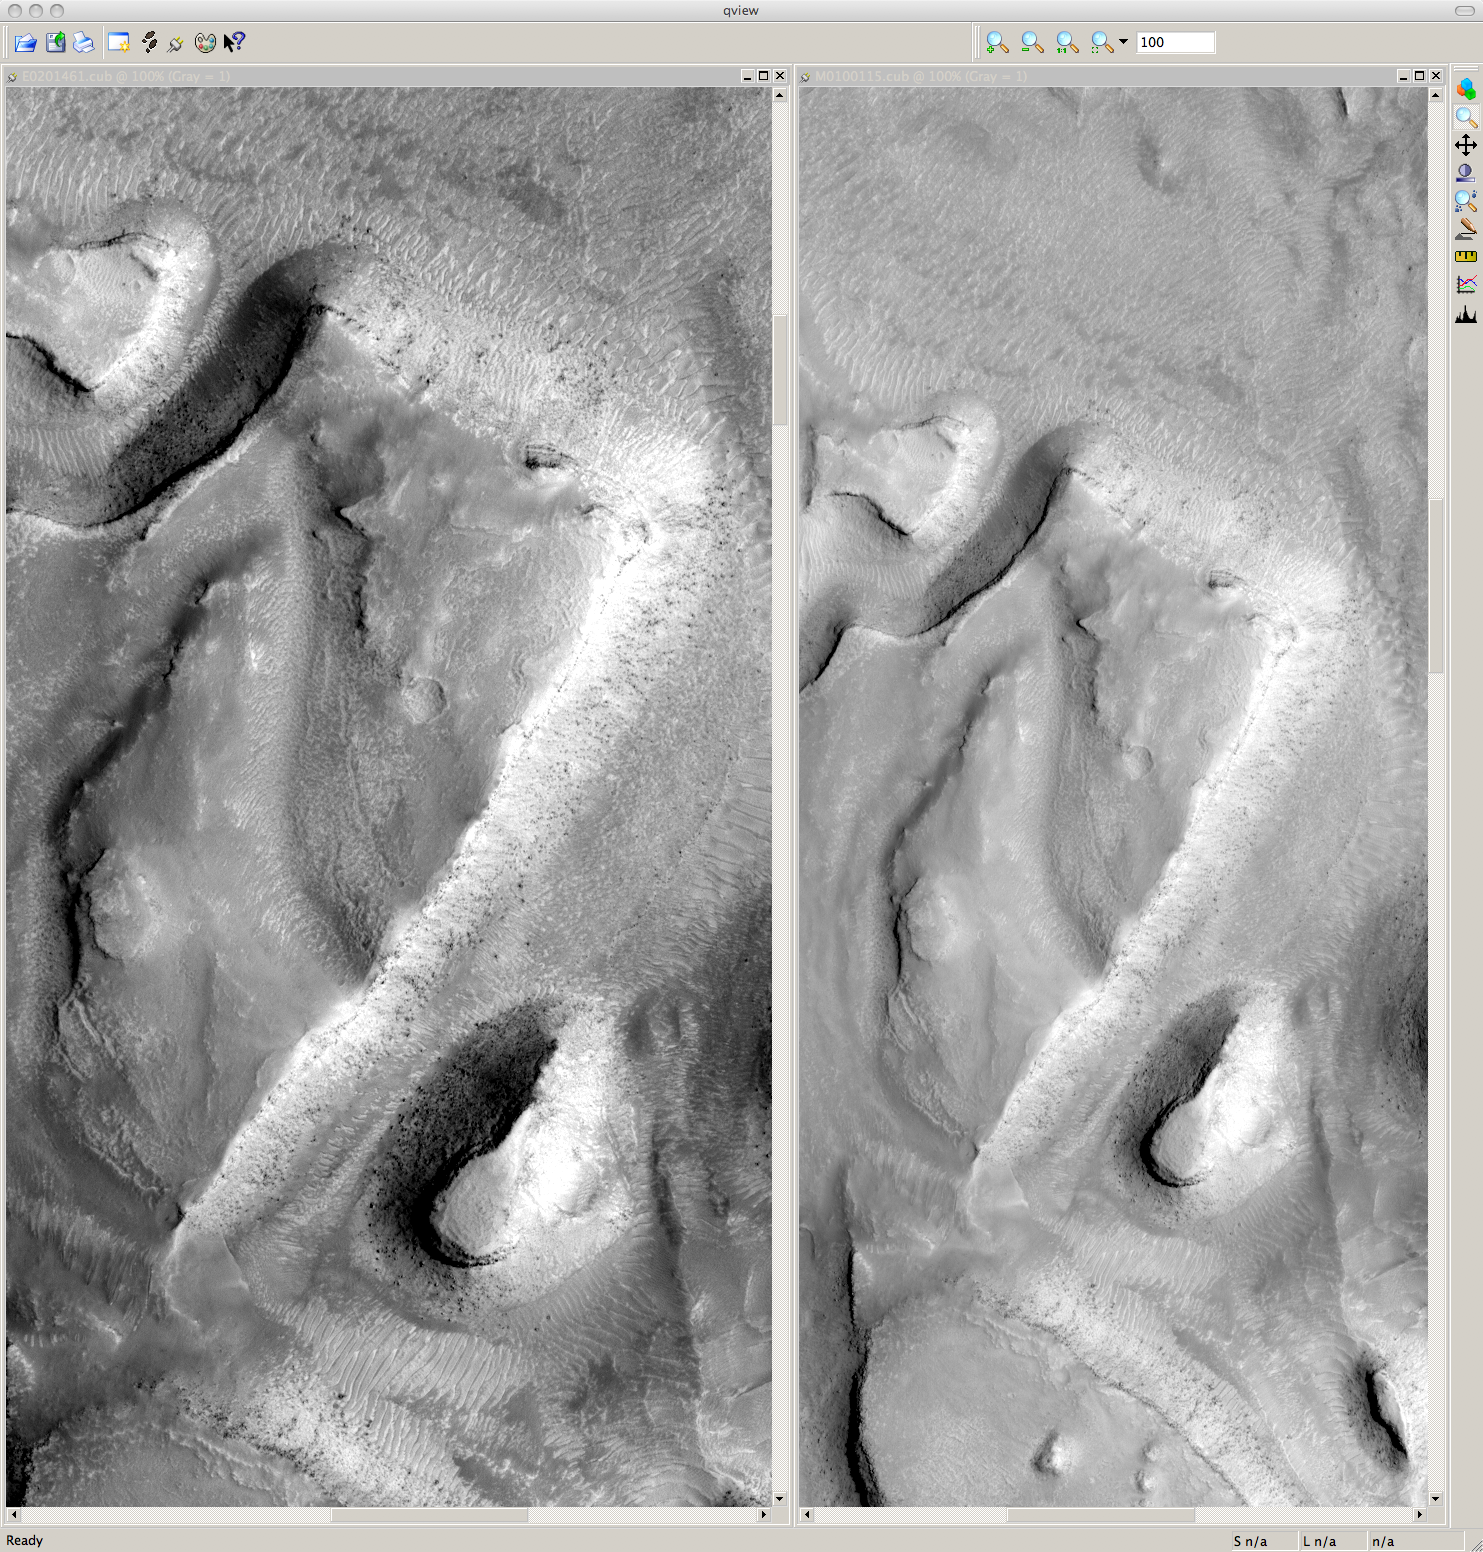
\includegraphics[height=3.7in]{images/p19-images_zoom.png}
\end{minipage}
\hfill
\begin{minipage}{1.3in}
\caption[P19 images open in qview zoomed in]{
    \label{p19-images}
    This shows \texttt{E0201461.cub} and \texttt{M0100115.cub} open in
        ISIS's qview program.  The view on the left shows their full extents
        at the same zoom level, showing how they have different ground scales.
        The view on the right shows them both zoomed in on the same feature.
    }
\end{minipage}
\end{figure}

% \section{Examples of Use}
%
% Download the tarball and it will unpack into a \texttt{p19} directory.  Create an output directory to hold the results, and invoke the \texttt{stereo} program:
%
% \begin{verbatim}
%       mkdir results
%       stereo E0201461.cub M0100115.cub results/p19
% \end{verbatim}
%
% You can look at the results by examining the disparity images. These
% show the horizontal and vertical components of the matching offsets
% for each pixel, and they can be a useful debugging tool if you want
% to check how the stereo matcher performed for a given stereo pair:
%
% \begin{verbatim}
%       cd results
%       disparitydebug p19-D.exr -o p19-D
%       disparitydebug p19-F.exr -o p19-F
% \end{verbatim}
%
% \emph{MJB: What exactly is being examined in the resultant images, what are users looking for?}
%
% A 3D mesh can be built from the point cloud and viewed using the
% \texttt{osgviewer} program:
%
% \begin{verbatim}
%       point2mesh p19-PC.tif p19-L.tif -o p19
%       osgviewer p19.ive
% \end{verbatim}
%
% When the \texttt{osgviewer} starts, you may want to turn off the
% lighting (hit the `L' key).
%
% A gridded DEM with floating point pixels can also be built from the point cloud:
%
% \begin{verbatim}
%       point2dem --xyz-to-lonlat -r mars p19-PC.tif -n -o p19
% \end{verbatim}
%
% You can also orthoproject the raw satellite imagery onto the DEM during this step:
%
% \begin{verbatim}
%       point2dem --xyz-to-lonlat -r mars p19-PC.tif -o p19 --orthoimage p19-L.tif
% \end{verbatim}
%
% Finally, you can create colorized, shaded relief (or both) images from the DEM, using these Vision Workbench programs:
%
% \begin{verbatim}
%       colormap p19-DEM.tif -o p19-colorized.tif
%       hillshade p19-DEM.tif -o p19-shaded.tif -e 25
%       colormap p19-DEM.tif --shaded-relief-file p19-shaded.tif -o p19-color-shaded.tif
% \end{verbatim}
%
% Finally, you can run the Vision Workbench's \texttt{image2qtree} on any of the following files:
%
% \begin{itemize}
% \item p19-DEM-normalized.tif
% \item p19-DRG.tif
% \item p19-shaded.tif
% \item p19-colorized.tif
% \item p19-shaded-colorized.tif
% \end{itemize}


\section{Tutorial}

The following example will utilize images from the example MOC
dataset, discussed above.  The two example ISIS 3 image files are
\texttt{E0201461.cub} and \texttt{M0100115.cub}.

The \texttt{stereo} program (page \pageref{stereo}) is designed for
automated tie point matching and stereo production, and is the first
Stereo Pipeline tool we'll use.

If you like, you should create a directory for the results of the
processing.  The \texttt{stereo} program can generate a number of
output files, and we find it helpful to put them all in a directory,
but it isn't required.

\begin{verbatim}
    > ls
    E0201461.cub   M0100115.cub
    > mkdir results
\end{verbatim}
\noindent
The \texttt{stereo} program requires a \texttt{stereo.default} file
which can be altered for your needs.  Its contents are detailed on
page \pageref{stereo.default}.  You may find it useful to save
multiple versions of the \texttt{stereo.default} file for various
processing needs. If you need to do that, be sure to specify which
configuration file \texttt{stereo} should use with the \texttt{-s}
option.  If this option is not given, the \texttt{stereo} program
will search for a file named \texttt{stereo.default} in the current
directory and will complain if there isn't one.

There is a \texttt{stereo.default} file included with the example
data set that is different from the example \texttt{stereo.default.example}
file distributed with the Stereo Pipeline.  The \texttt{stereo.default}
included with the example data set has a smaller correlation window
(smaller values for the \texttt{H\_CORR\_*} and \texttt{V\_CORR\_*}
variables) that is more suited to the MOC data.  You may want to
use both this \texttt{stereo.default} and the
\texttt{stereo.default.example} to explore how the results are
different.

So run \texttt{stereo} like this (there should be a
\texttt{stereo.default} file distributed along with the example
data set that will be used):

\begin{verbatim}
    ISIS 3> stereo E0201461.cub M0100115.cub results/E0201461-M0100115
\end{verbatim}
\noindent
So that last text can be anything you want it to be.  It designates
the text that \texttt{stereo} will use as a prefix for its many
output files.  Since the first part is \texttt{results/} this causes
the program to put the results in that directory with files whose
names start with \texttt{E0201461-M0100115}.  If instead that last
text was just \texttt{E0201461-M0100115} it would have created a
bunch of files that start with \texttt{E0201461-M0100115} in the
same directory as the input files.

The \texttt{stereo} program's processing moves through several
stages which are detailed on page \pageref{entrypoints}.  However,
once the \texttt{stereo} program completes, it creates a number of
files.  A quick look at some of the TIFF files created, can quickly
give you an idea of what the \texttt{stereo} program did (figure
\ref{p19-stereo-output}).


\begin{figure}
\begin{center}
\includegraphics[width=5in]{images/p19-stereo-output.png}
\caption[P19 stereo output images]{
    \label{p19-stereo-output}
	These are the four viewable \texttt{.tif} files created by
	the \texttt{stereo} program.  The left two are the aligned
	images (\texttt{E0201461-M0100115-L.tif} and
	\texttt{E0201461-M0100115-R.tif}).  The next two images are
	the mask images (\texttt{E0201461-M0100115-lMask.tif} and
	\texttt{E0201461-M0100115-rMask.tif}), which indicate which
	pixels in the aligned images are good to use for the next
	step.  The image on the right is the Good Pixel map
	(\texttt{E0201461-M0100115-GoodPixelMap.tif}), which indicates
	the pixels in grey which were successfully matched with the
	correlator.  The red pixels were not.  Those red pixels which
	are not black in both mask images are optionally filled later
	during the hole-filling step.
    }
\end{center}
\end{figure}

% \begin{figure}
% \begin{center}
% 
\includegraphics[height=8in]{images/p19-goodpixel.png}
% \caption[P19 good pixel image]{
%     \label{p19-goodpixel}
% 	The Good Pixel map.
% 	Red pixels are not useful for alignment.
%     }
% \end{center}
% \end{figure}
%
% \begin{figure}
% \begin{center}
% 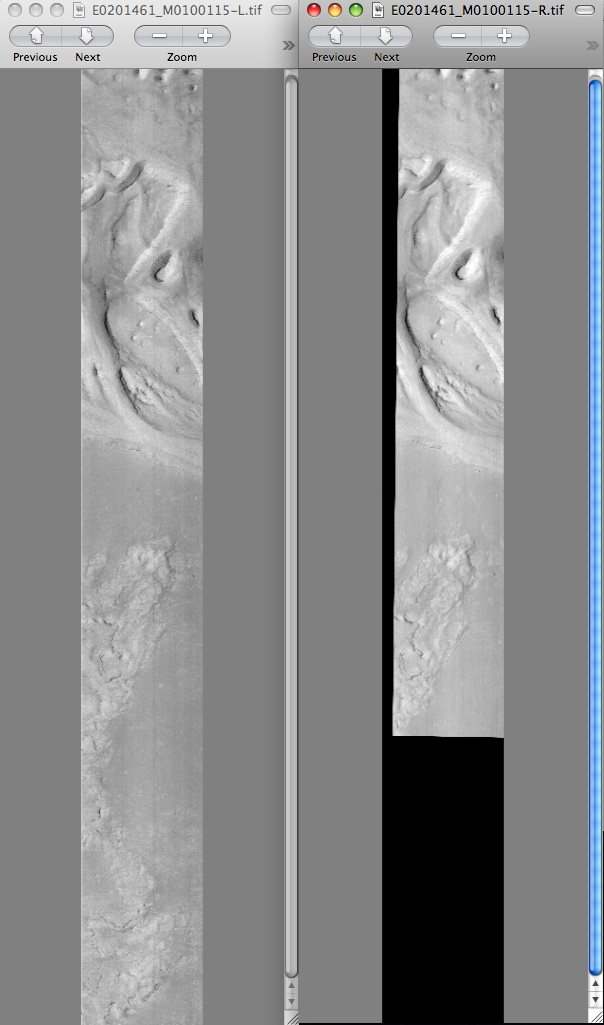
\includegraphics[width=3in]{images/p19-aligned.png}
% \caption[P19 aligned image]{
%     \label{p19-aligned}
% 	The left and right aligned images.
%     }
% \end{center}
% \end{figure}

If those TIFF files look okay, you can probably just go on to making
a mesh or a DTM from the point cloud file
(\texttt{E0201461-M0100115-PC.tif}).  The most important file is
the Good Pixel Map (\texttt{E0201461-M0100115-GoodPixelMap.tif}).
If this file shows mostly good, gray pixels in the overlap area
(the area that is white in both the \texttt{E0201461-M0100115-lMask.tif}
and \texttt{E0201461-M0100115-rMask.tif} files), then you're probably
good to go.  If this shows bad, red pixels in the overlap area,
then you'll probabaly need to go back and tune your \texttt{stereo.default}
file.  The example data also contains a \texttt{stereo.bad} file
which has intentionally bogus values for the dimensions of the
correlation window.  You can run \texttt{stereo} with the \texttt{-s
stereo.bad} command to see what the Good Pixel Map looks like with
this.

To get an idea of the disparity information that the \texttt{stereo}
program created and then used to build the point cloud, it can be
useful to take a look at that disparity information.  The \texttt{stereo}
program records this information in several \texttt{.exr} disparity
files.

To get a look at the disparity information, you need to convert it
into a more viewable format.  Move into the directory that contains
your results, and run the \texttt{disparitydebug} program (page
\pageref{disparitydebug}) to create the the horizontal and vertical
components of the disparity (matching offsets for each pixel).

\begin{figure}[b!]
\begin{minipage}{4in}
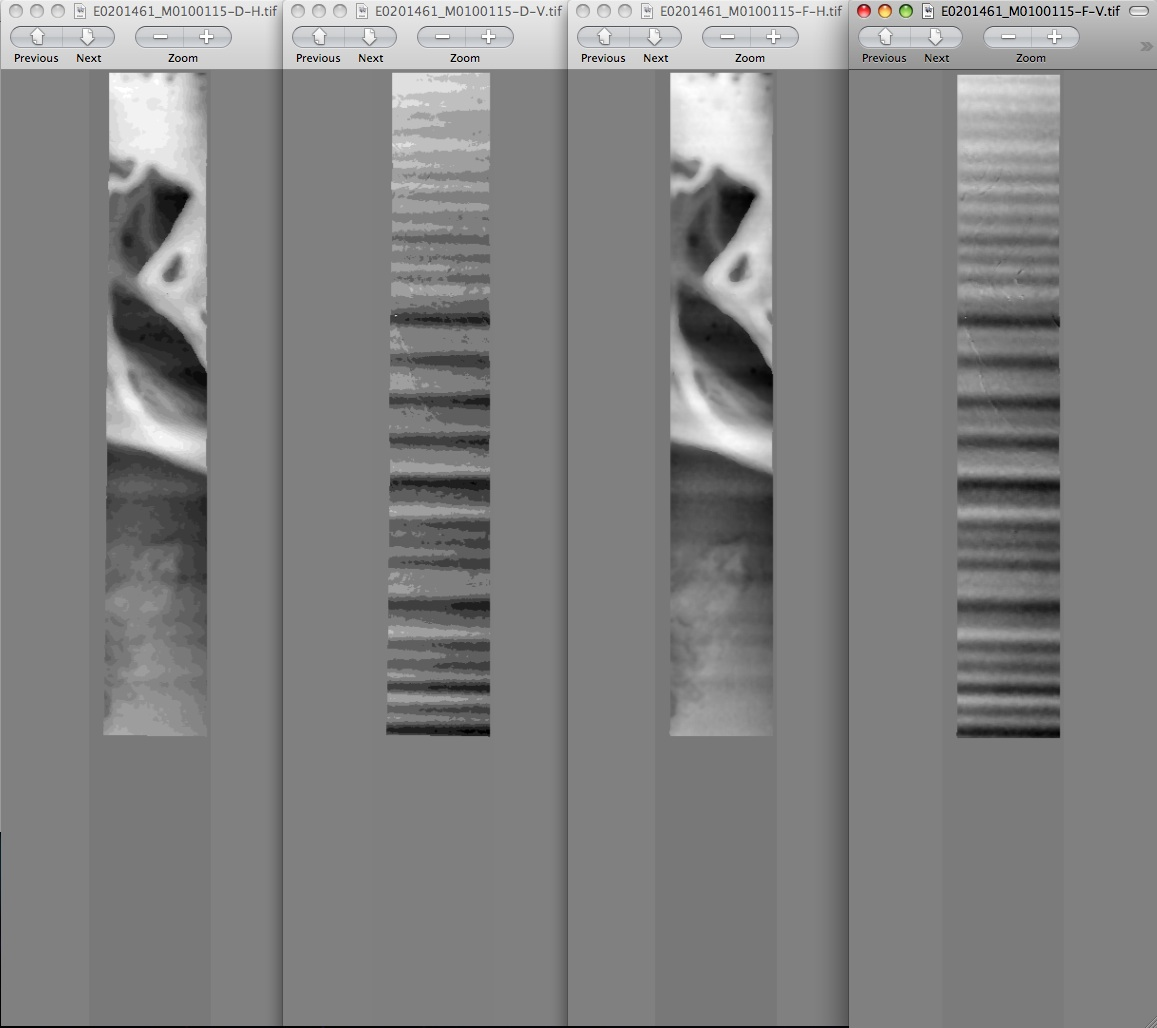
\includegraphics[width=4in]{images/p19-disparity.png}
\end{minipage}
\hfill
\begin{minipage}{2.7in}
\caption[P19 disparity images]{
    \label{p19-disparity}
	The disparity images.  The two images on the left are the
	\texttt{E0201461-M0100115-D-H.tif} and
	\texttt{E0201461-M0100115-D-V.tif} files, which are the raw horizontal and
	vertical disparity components.  The two images on the right are the
	\texttt{E0201461-M0100115-F-H.tif} and
	\texttt{E0201461-M0100115-F-V.tif} files, which are the final
	filtered, sub-pixel disparity map with outlier removal and holes
	filled in, and is what will be used to build the point cloud.  Since
	these MOC images were acquired by rolling the spacecraft across-track,
	most of the disparity that represents topography is present in the
	horizontal disparity map.  The vertical disparity map shows disparity
	not from topography, but from spacecraft movement.
    }
\end{minipage}
\end{figure}

\begin{verbatim}
    cd results
    disparitydebug E0201461-M0100115-F.exr
\end{verbatim}
\noindent
The two output files, \texttt{E0201461-M0100115-F-H.tif} and
\texttt{E0201461-M0100115-F-V.tif} are normalized images of the
horizontal (H) and vertical (V) disparity.  `Normalized' is a key
word here.  You can see that the horizontal and vertical disparity
images in figure \ref{p19-disparity} have the same range of gray
values from white to black, but they represent significantly different
absolute amounts of disparity.  These files are useful if you want
to check the performance of the \texttt{stereo} program for any
given stereo pair.

There are actually four flavors of disparity map: the \texttt{-D.exr},
the \texttt{-R.exr}, the \texttt{-F-corrected.exr}, and \texttt{-F.exr}.
You can run \texttt{disparitydebug} on any of them, and actually taking a
look at all of them can show you the differences between the disparity maps
at the different stages of processing.

At this point, the processing fans out, as many kinds of data
products can be built from the \texttt{E0201461-M0100115-PC.tif}.

One of the things that can be done is to produce a 3D mesh with
\texttt{point2mesh} (page \pageref{point2mesh}).  This image can
be viewed with \texttt{osgviewer} (the Open Scene Graph Viewer
program, distributed with the binary version of the Stereo Pipeline).
The \texttt{point2mesh} program takes the point cloud file and one
of the image files (usually the highest resolution one) created by
\texttt{stereo} as inputs.

\begin{verbatim}
    point2mesh E0201461-M0100115-PC.tif E0201461-M0100115-L.tif
\end{verbatim}
\noindent
This will create the file \texttt{E0201461-M0100115.ive}, openable
with \texttt{osgviewer}. When the \texttt{osgviewer} program starts,
you may want to turn off the lighting (hit the `L' key).

\begin{figure}[h]
\begin{minipage}{5in}
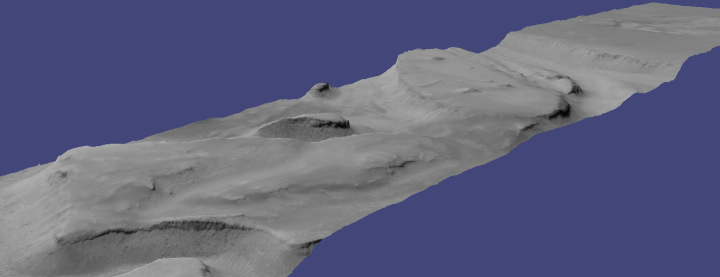
\includegraphics[width=5in]{images/p19-osg.png}
\end{minipage}
\hfill
\begin{minipage}{1.7in}
\caption[P19 in OSG]{
    \label{p19-osg}
	This shows the \texttt{E0201461-M0100115.ive} file displayed in
	the OSG Viewer.
    }
\end{minipage}
\end{figure}

The \texttt{point2dem} program (page \pageref{point2dem}) creates
a digital elevation model (DEM) from the Point Cloud file.

\begin{verbatim}
    point2dem E0201461-M0100115-PC.tif
\end{verbatim}

The resultant file, \texttt{E0201461-M0100115-DEM.tif}, will have
32-bit pixels, and so (much like the \texttt{E0201461-M0100115-PC.tif}
file) will not render well in typical image viewers.

You can specify a coordinate system (e.g., latlon) and a reference
spheroid (i.e., calculated for the Moon or Mars). You also have the
option of creating a normalized DEM in addition to the automatically
generated non-normalized DEM.

\begin{verbatim}
    point2dem --xyz-to-lonlat -r mars -n E0201461-M0100115-PC.tif
\end{verbatim}
\noindent
The \texttt{point2dem} program can also be used to orthoproject raw
satellite imagery onto the DEM. To do this, invoke \texttt{point2dem}
just as before, but add the \texttt{orthoimage} option and specify
the use of the left image file as the texture file to use for the
projection

\begin{verbatim}
    point2dem --xyz-to-lonlat -r mars --orthoimage E0201461-M0100115-L.tif \
      E0201461-M0100115-PC.tif
\end{verbatim}
\noindent
The \texttt{point2dem} program can be used in many different ways.
Be sure to explore all of the options.

\begin{figure}
\begin{minipage}{4in}
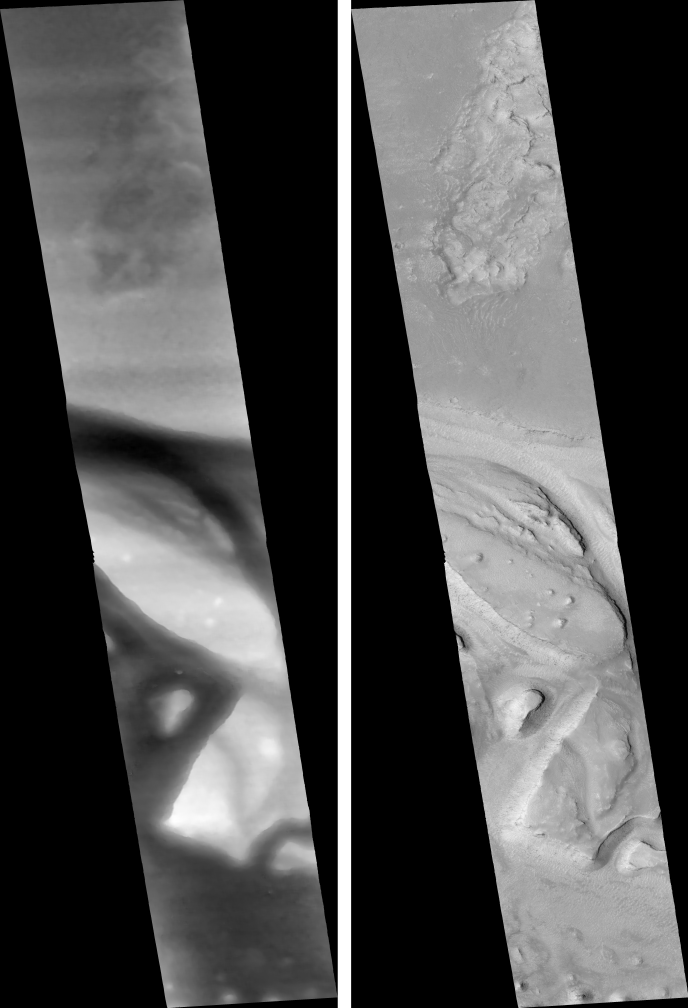
\includegraphics[width=4in]{images/p19-norm_ortho.png}
\end{minipage}
\hfill
\begin{minipage}{2.7in}
\caption[P19 Normalized DEM and Orthophoto]{
    \label{p19-norm_ortho}
	The image on the left is a normalized DEM (using the
	\texttt{-n} option) which which shows low terrain values
	as black and high terrain values as white (in a 0 to 255
	sense).  The image on the right is the orthographic image
	(created using the \texttt{--orthoimage} option to
	\texttt{point2dem}).
    }
\end{minipage} \end{figure}

% \begin{figure}
% \begin{center}
% 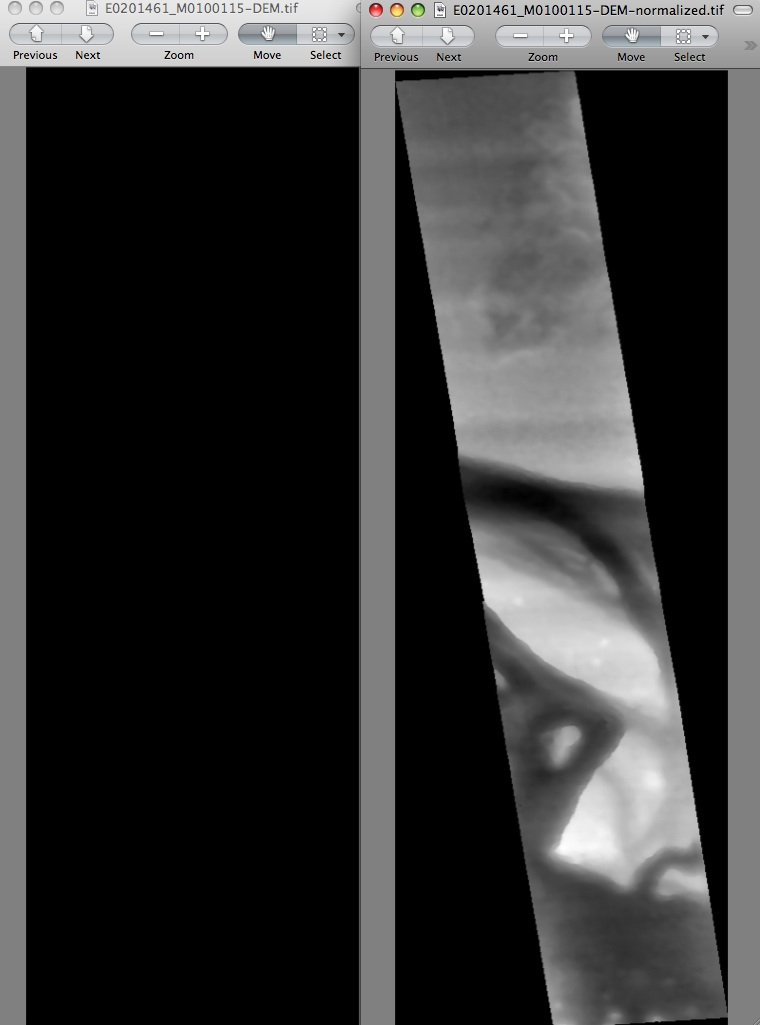
\includegraphics[width=4in]{images/p19-dems.png}
% \caption[P19 dem images]{
%     \label{p19-dems}
% 	The non-normalized and normalized DEMs. Note that the
% 	non-normalized version contains floating point pixel values
% 	and will not open in most image viewing programs which
% 	expect integer pixel values between 0 and 255 (which is
% 	what the normalized version does for you).
%     }
% \end{center}
% \end{figure}
%
% \begin{figure}
% \begin{center}
% \includegraphics[width=3in]{images/p19-ortho.png}
% \caption[P19 orthophoto]{
%     \label{p19-ortho}
% 	The left image orthoprojected onto the DEM.
%     }
% \end{center}
% \end{figure}

Once you have generated a DEM, you can use the Vision Workbench's
\texttt{colormap} and \texttt{hillshade} tools to create colorized
and/or shaded relief images from the DEM.

To create a colorized version of the DEM, you need only specify the
DEM file to use:

\begin{verbatim}
    colormap p19-DEM.tif -o p19-colorized.tif
\end{verbatim}

To create a hillshade of the DEM, you should specify the DEM file
to use. It is also advisable to explore the effects of altering the
elevation of the light source.

\begin{verbatim}
    hillshade p19-DEM.tif -o p19-shaded.tif -e 25
\end{verbatim}

To create a colorized version of the shaded relief file, specify
the DEM and the shaded relief file that should be used.

\begin{verbatim}
    colormap p19-DEM.tif --shaded-relief-file p19-shaded.tif -o p19-color-shaded.tif
\end{verbatim}

\begin{figure}
\begin{center}
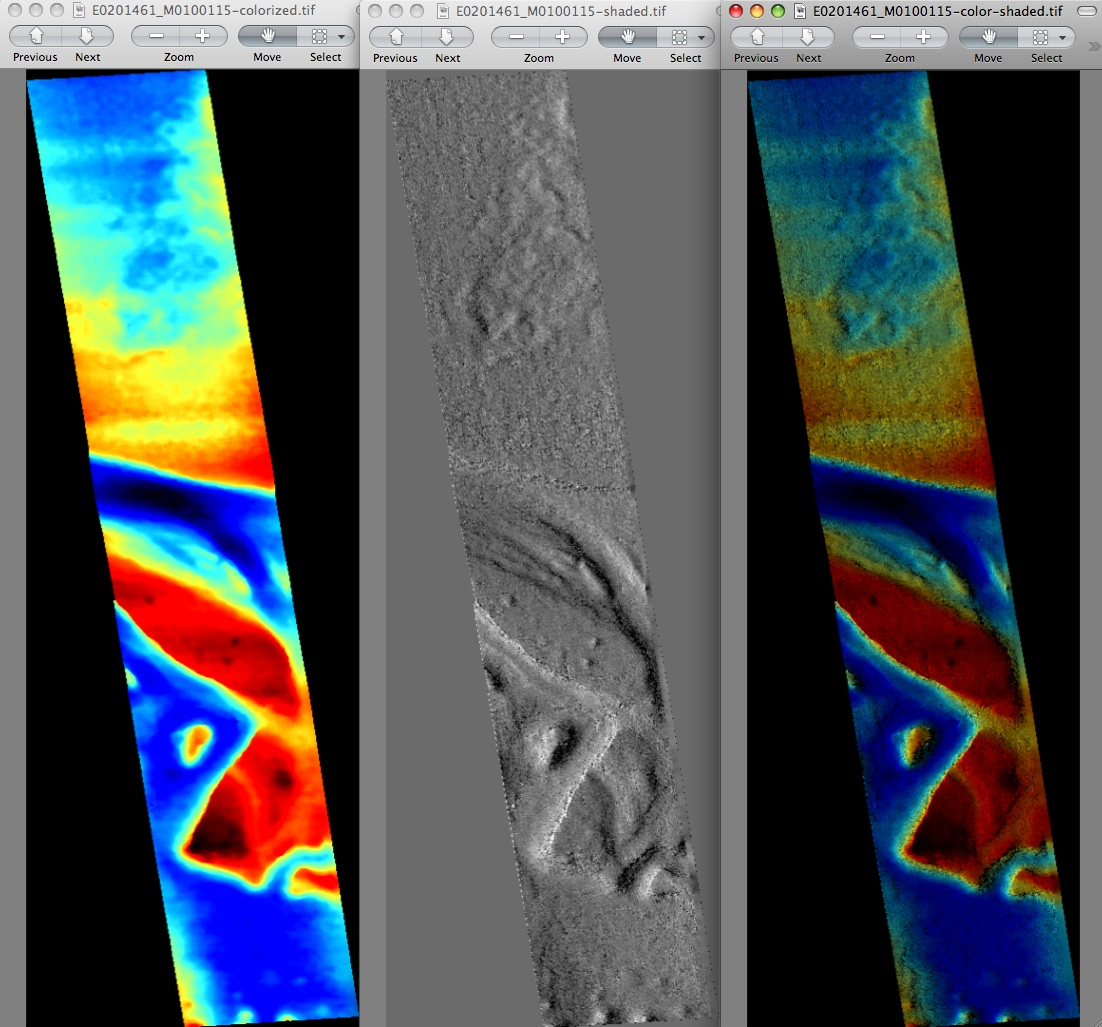
\includegraphics[width=5in]{images/p19-colorized-shaded.png}
\caption[P19 colorized and shaded relief]{
    \label{p19-color}
	The colorized DEM, the shaded relief image, and the colorized hillshade.
    }
\end{center}
\end{figure}

The final option of the stereo processing package is \texttt{image2qtree}.
This function was designed for use in creating geographically
referenced images in tiles such that each tile can be viewed at
ideal resolution.

The \texttt{image2qtree} program can be used on any of the following files that you
have generated:
\begin{verbatim}
    p19-DEM-normalized.tif
    p19-DRG.tif
    p19-shaded.tif
    p19-colorized.tif
    p19-shaded-colorized.tif
\end{verbatim}

Specify which image you would like to invoke \texttt{image2qtree} on, along
with any combination of options.

\begin{verbatim}
    image2qtree p19-DEM-normalized.tif -o p19-DEM-n-qtree
\end{verbatim}


%% \section{Preparing Selected Data}

%% There are many ways to process different kinds of image data, and
%% some will be more appropriate for operations by the Stereo Pipeline
%% than others.  While we strive to make the Stereo Pipeline extensible
%% and robust, there are a limited (but growing) set of data that we
%% have thoroughly tested.

%% This section outlines the suggested pre-processing steps to prepare
%% specific data sets for use in the Stereo Pipeline.

%% \subsection{Mars Oribiter Camera (MOC)}

%% MOC images (ending in \texttt{.imq} or \texttt{.img}) can be downloaded from
%% the PDS and only require a single ISIS command to prepare for Stereo Pipeline use:

%% \begin{verbatim}
%%     ISIS 3> mocproc from= MOCimage.imq to= MOCimage.cub Mapping= NO
%% \end{verbatim}

%% The resulting ISIS cube file (e.g. \texttt{MOCimage.cub}) is now ready
%% for processing by the \texttt{stereo} program.


%% \subsection{High Resolution Imaging Science Experiment (HiRISE)}

%% HiRISE images are more complicated.

%% At the moment, the `best' processing method is to start with HiRISE
%% \texttt{*.balance.cub} files (available only internally to the
%% HiRISE team) and run them through the USGS's \texttt{hinoproj.pl}
%% script.  This results in \texttt{noproj}ed and de-jittered cube
%% files that can be run.

%% In the future (who knows when), the HiRISE team will directly produce
%% \texttt{noproj}ed images (dejittered through a different, improved,
%% algorithm) which will be available in the \texttt{extras/} directory
%% of the HiRISE PDS Volume.  And those images will probably be directly
%% usable by the Stereo Pipeline.

%% \emph{As you can tell, I'm still in the process of tracking all of this down. -RAB}

\chapter{Programs}

This chapter covers the various user-programs that are a part of
the Ames Stereo Pipeline.

\section{stereo}

The \texttt{stereo} program is the primary workhorse of the Ames
Stereo Pipeline.  It is the program that takes a pair of images which
overlap and creates an output point cloud which can then be fed to the
\texttt{point2mesh} or \texttt{point2dem} programs.

\emph{Way more needs to go in here ...}

\subsection{stereo.default file}

The \texttt{stereo.default} file contains configuration parameters
which the \texttt{stereo} program uses to process the images.  Below
we will walk through the contents of the \texttt{stereo.default.example}
file distributed with the Ames Stereo Pipeline and discuss all of
the various parameters.

The parameters which begin with `\texttt{DO\_}' are true/false options,
when set to `1' they are `on' or `true,' and if set to `0' they are
`off' or `false.'

The parameters below also have their default values listed after
the parameter name.

\subsubsection*{Preprocessing}

\begin{description}
\item[DO\_INTERESTPOINT\_ALIGNMENT 1] \hfill \\
When \texttt{DO\_INTERESTPOINT\_ALIGNMENT} is on (or set to 1), ... \emph{MJB: describe}

\item[DO\_EPIPOLAR\_ALIGNMENT 0] \hfill \\
By default this is off.  When on ... \emph{MJB: describe}

\item[INTERESTPOINT\_ALIGNMENT\_SUBSAMPLING 1] \hfill \\
This option allows you to change the density of interest points
that stereo will find, correlate, and result in the final point
cloud.  When this is set to 1, there is no subsampling, the
\texttt{stereo} program will do its best to find as many interest
points within the imagery as it can.  When this is set to 2, the
program will ignore every other interest point that it finds, and
will only process the reduced set.  This parameter can be set to
any positive integer.  When this parameter is turned up, the resulting
point cloud will have less effective resolution.

\item[DO\_SLOG 1 and DO\_LOG 0] \hfill \\
These two items are related, only one can be set to `on', if both
are `on' the program will default to doing only SLOG.  \emph{MJB: explain the difference}

\item[SLOG\_KERNEL\_WIDTH 1.5] \hfill \\
When \texttt{DO\_SLOG} is `on,' this option sets the diameter of
the convolution kernel. \emph{MJB: describe}

\end{description}

\subsubsection*{Correlation}
\subsubsection*{Filtering}
\subsubsection*{Dot Cloud}

\section{disparitydebug}
\section{results}
\section{point2mesh}
\section{point2dem}
\section{orthoproject}

\chapter{Bundle Adjustment}
\label{ch:bundle_adjustment}

\newenvironment{myindentpar}[1]
               {\begin{list}{}
                   {\setlength{\leftmargin}{#1}}
                 \item[]
               }
               {\end{list}}

\definecolor{lgray}{gray}{0.95}

Satellite position and orientation errors have a direct effect on the
accuracy of digital elevation models produced by the Stereo Pipeline.
If they're not corrected, these uncertainties will result in
systematic errors in the overall position and slope of the \ac{DEM}.
Severe distortions can occur as well, resulting in twisted or ``taco
shaped'' \acp{DEM}, though in most cases these effects are quite
subtle and hard to detect. In the worse case, such as with old mission
data like Voyager or Apollo, these gross camera misalignments can
prohibit Stereo Pipeline's internal interest point matcher and block
auto search range detection.

USGS's \ac{ISIS} software contains a suite of tools for correcting camera
position and orientation errors for their cameras using a process
called \emph{bundle adjustment}. Bundle adjustment is the process of
simultaneously adjusting the properties of many cameras and the 3D
locations of the objects they see in order to minimize the error
between the estimated, back-projected pixel location of the 3D objects
and their actual measured location in the captured images.

That complex process can be boiled down to this simple idea: bundle
adjustment ensures that observations in multiple different images of a
single ground feature are self-consistent. If they are not consistent,
then the position and orientation of the cameras as well as the 3D
position of the feature must be adjusted until they are.  This
optimization is carried out along with thousands (or more) of similar
constraints involving many different features observed in other
images.  Bundle adjustment is very powerful and versatile: it can
operate on just two overlapping images, or on thousands. It is also a
dangerous tool. Careful consideration is required to insure and
verify that the solution does represent reality.

\begin{figure}[bt]
  \centering
  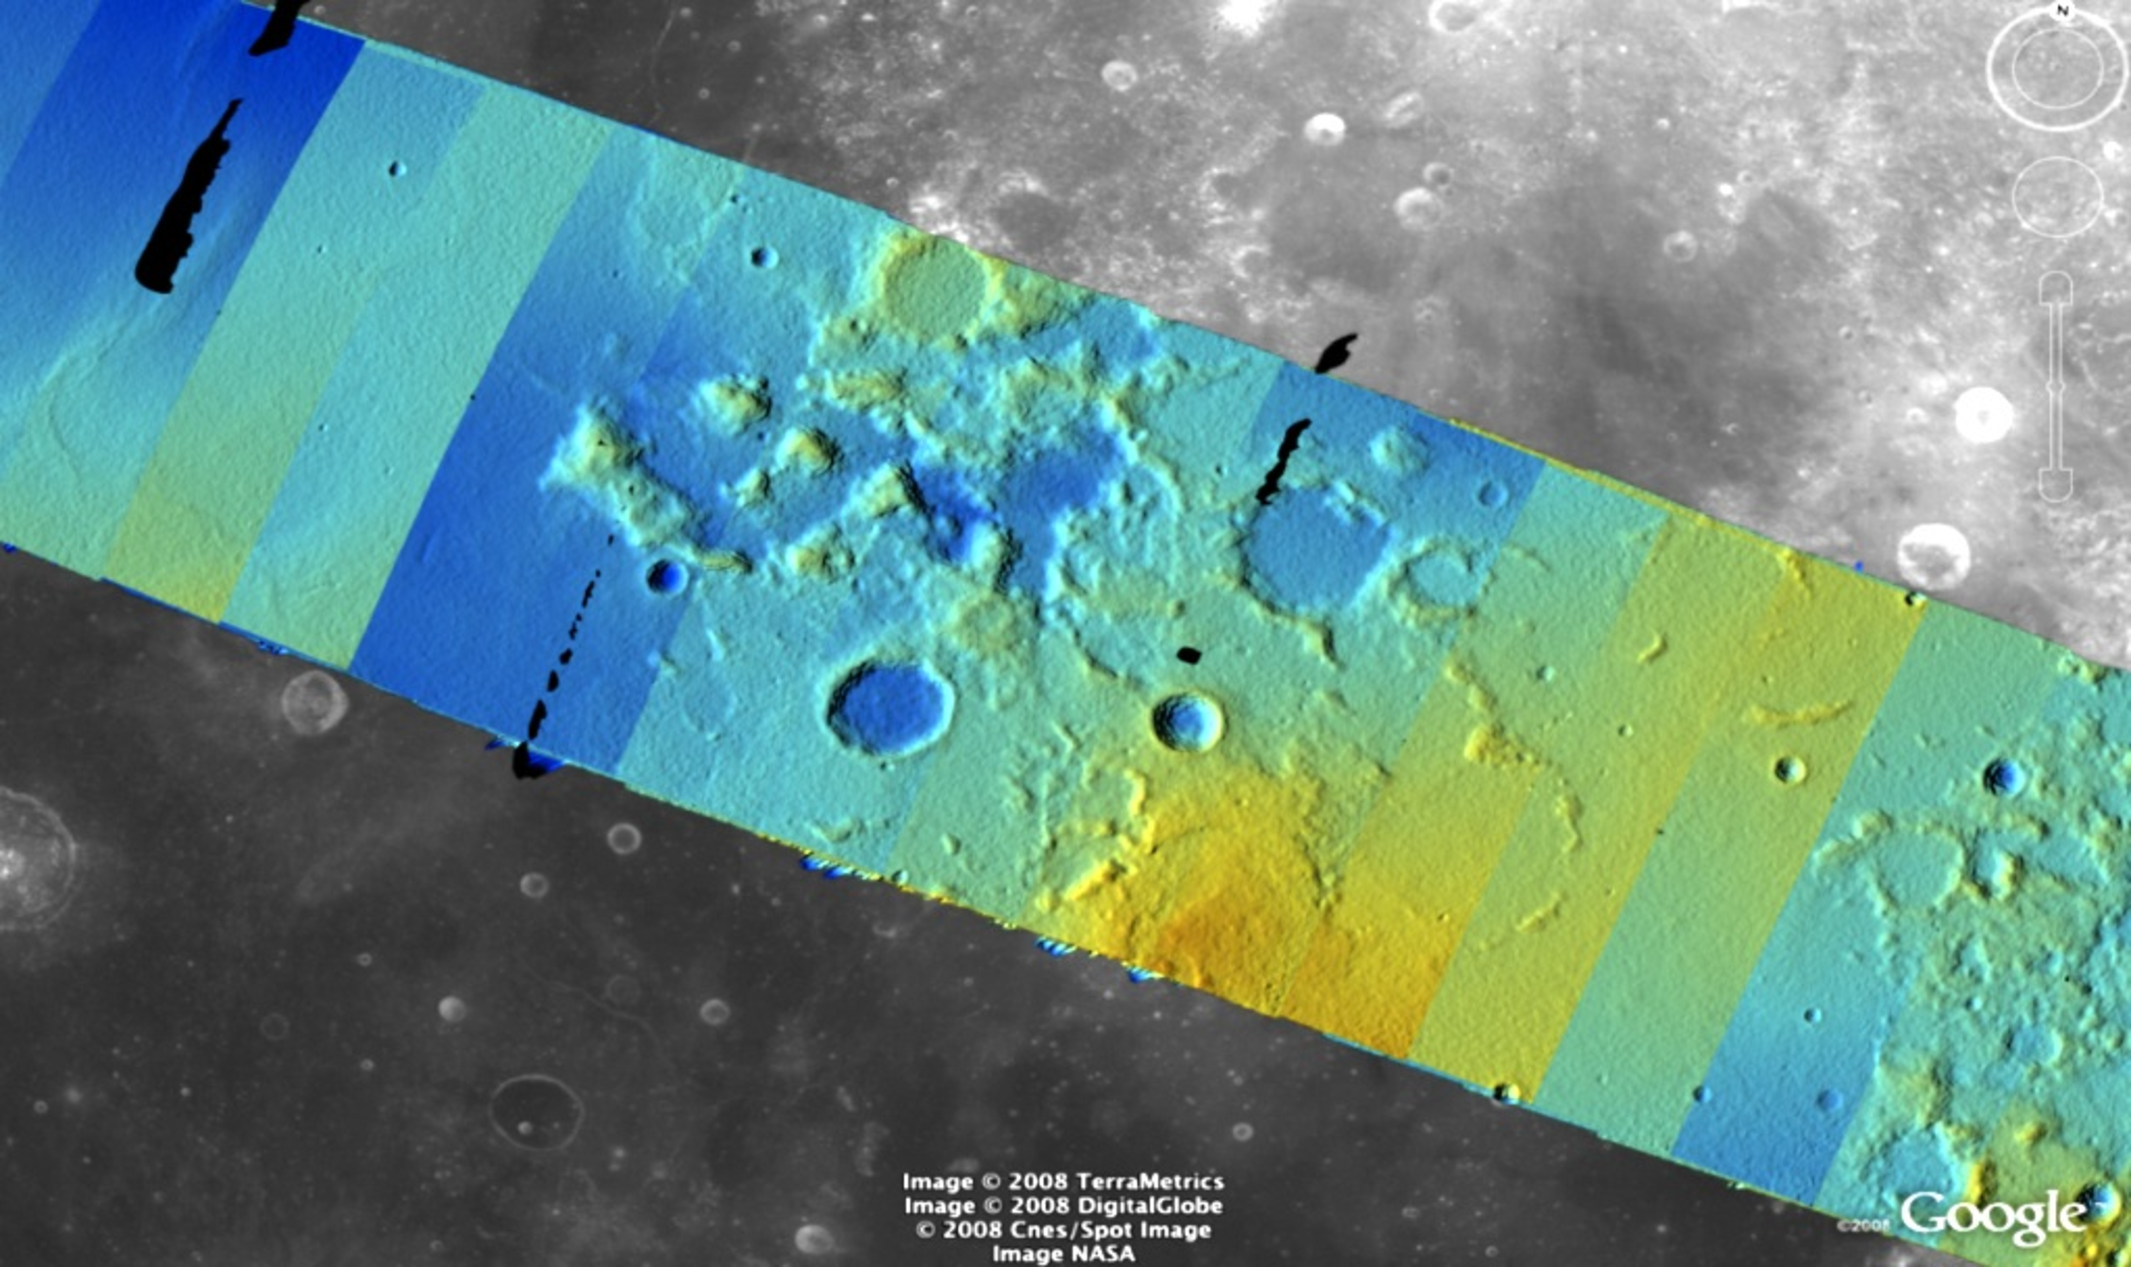
\includegraphics[width=8cm]{images/ba_orig}
  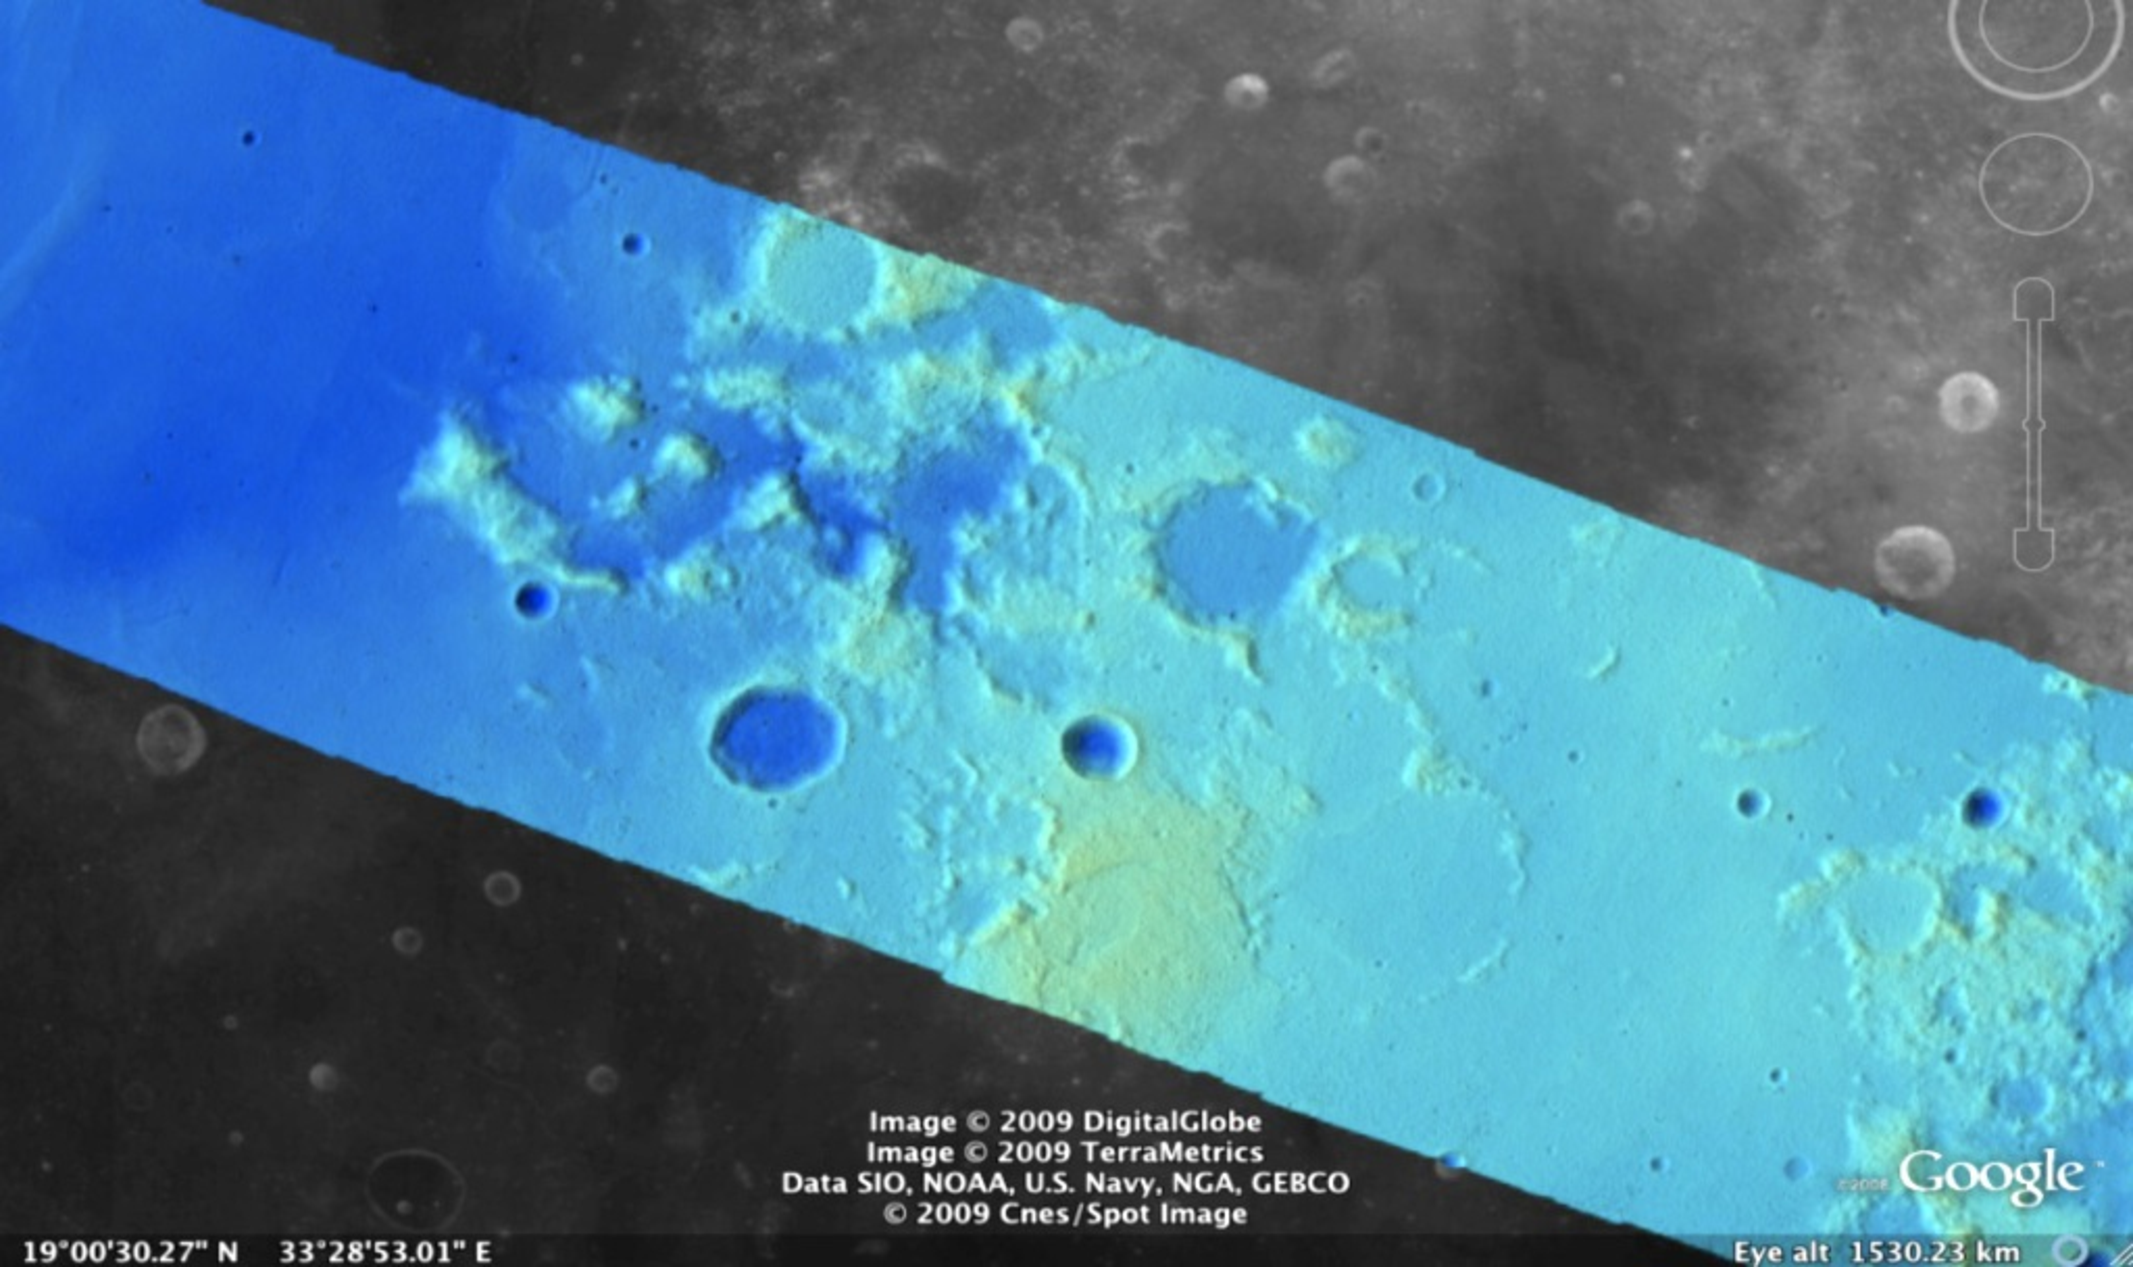
\includegraphics[width=8cm]{images/ba_adjusted}
  \caption{Bundle adjustment is illustrated here using a color-mapped,
    hill-shaded DEM mosaic from Apollo 15, Orbit 33, imagery. (a)
    Prior to bundle adjustment, large discontinuities can exist between
    overlapping DEMs made from different images. (b) After bundle
    adjustment, DEM alignment errors are minimized, and no longer visible.}
  \label{fig:bundle_adjustment}
\end{figure}

Bundle adjustment can also take advantage of \acp{GCP}, which are
3D locations of features that are known apriori (often by measuring
them by hand in another existing \ac{DEM}). \acp{GCP} can improve the internal
consistency of your \ac{DEM} or align your \ac{DEM} to an existing data
product. Finally, even though bundle adjustment calculates the
locations of the 3D objects it views, only the final properties of
the cameras are recorded for use by the Ames Stereo Pipeline. Those
properties can be loaded into the \texttt{stereo} program which
uses its own method for triangulating 3D feature locations.

When using the Stereo Pipeline, bundle adjustment is an optional step
between the capture of images and the creation of \acp{DEM}. The bundle
adjustment process described below should be completed prior to
running the \texttt{stereo} command.

Although bundle adjustment is not a required step for generating
\acp{DEM}, it is {\em highly recommended} for users who plan to
create \acp{DEM} for scientific analysis and publication.  Incorporating
bundle adjustment into the stereo work flow not only results in
\acp{DEM} that are more internally consistent, it is also the correct
way to co-register your \acp{DEM} with other existing data sets and
geodetic control networks.

At the moment however, Bundle Adjustment does not automatically work
against outside DEMs from sources such as laser altimeters. Hand
picked \acp{GCP} are the only way for \ac{ASP} to register to those
types of sources.

\subsection{A deeper understanding}

In bundle adjustment the position and orientation of each camera
station are determined jointly with the 3D position of a set of image
tie-points points chosen in the overlapping regions between
images. Tie points, like they sound, tie individual camera images
together. Their physical manifestation would be a rock or small crater
than can be observed across multiple images.

Tie-points can be automatically extracted using Vision Workbench's
Interest Point module, \ac{ISIS}'s \texttt{autoseed} and \texttt{pointreg},
or through a number of outside methods such as the famous
SURF\citep{surf08}. We'll be discussing the method of gathering these
measurements using \ac{ISIS}'s toolchain. Creating a collection of tie
points, {\it called a control network}, is a three step process. First, a
general geographic layout of the points must be decided upon. This is
traditionally just a grid layout that has some spacing that allows for
about a 20-30 measurements to be made per image. This decided upon grid
shows up in slightly different projected locations each image due to
their slight misalignments. The second step is have an automatic
registration algorithm try to find the same feature in all images using
the prior grid as a starting location. The third step is to manually
verify all measurements visually, checking to insure that each
measurement is looking at the same feature.

\begin{figure}[b!]
  \begin{center}
  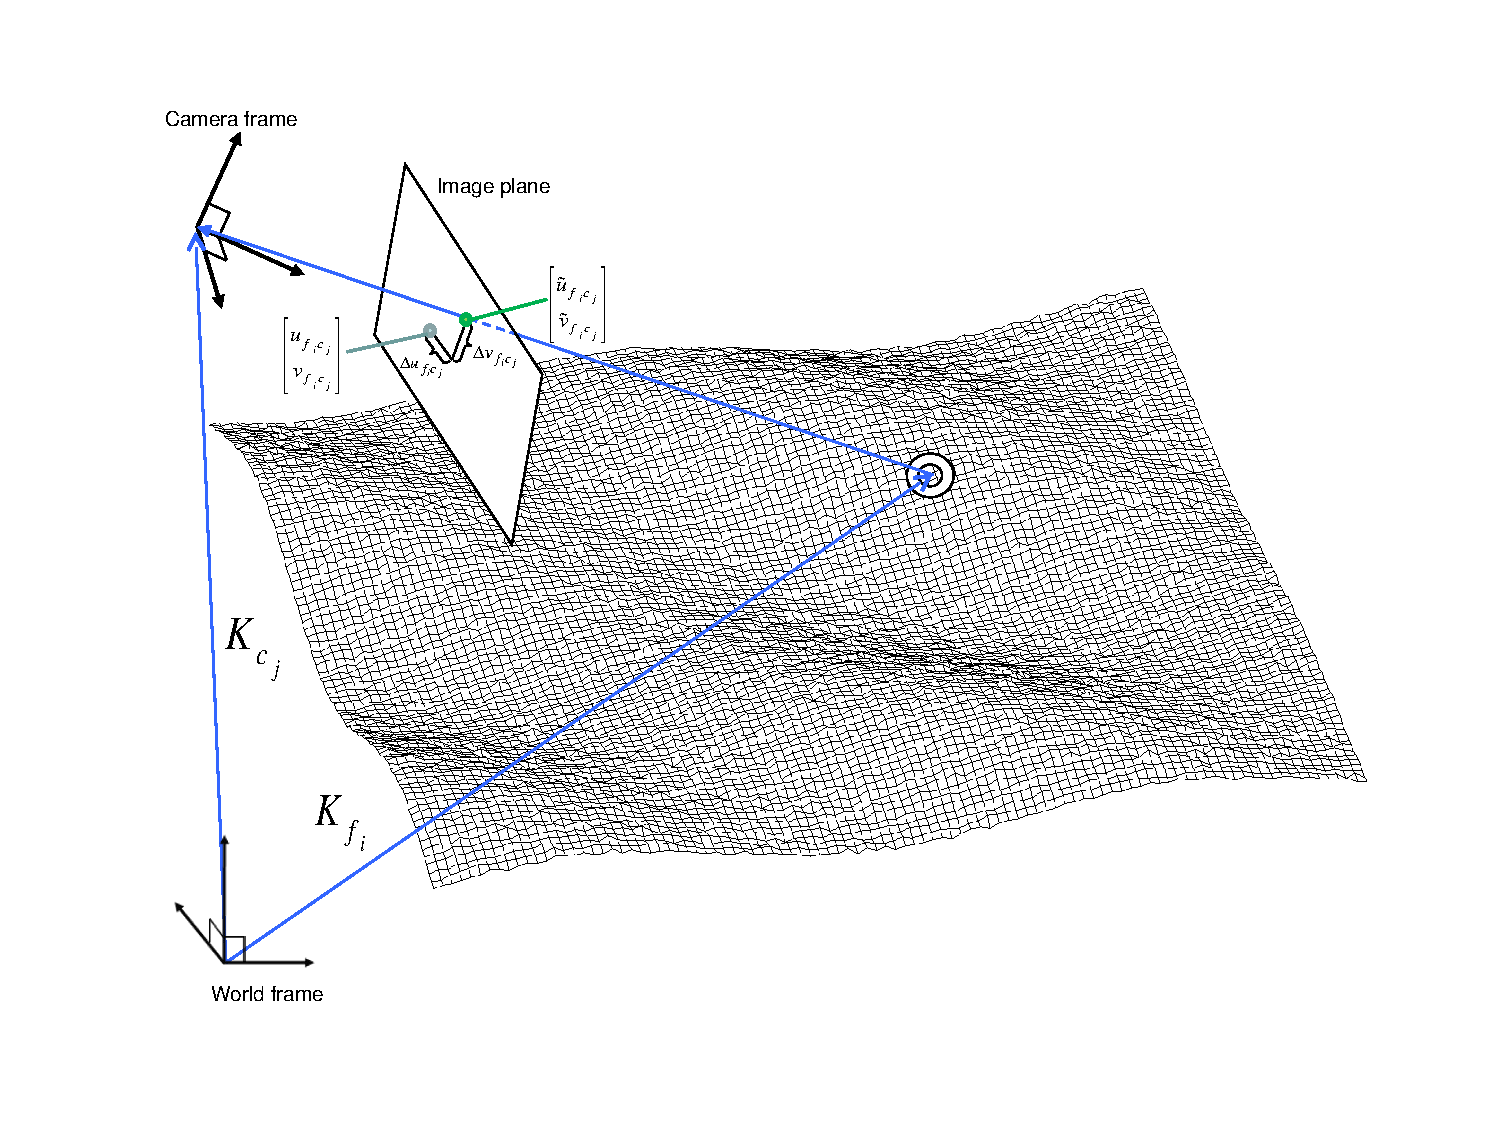
\includegraphics[trim=20mm 20mm 20mm 15mm,clip,width=6in]{images/ba_feature_observation.pdf}
  \end{center}
  \caption{ A feature observation in bundle adjustment, from \citet{moore09} }
  \label{fig:ba_feature}
\end{figure}

Bundle Adjustment in \ac{ISIS} is performed with the \texttt{jigsaw}
executable. It generally follows the method described
in~\cite{triggs00} and determines the best camera parameters that
minimize the projection error given by ${\bf \epsilon} =
\sum_k\sum_j(I_k-I(C_j, X_k))^2$ where $I_k$ are the tie points on the
image plane, $C_j$ are the camera parameters, and $X_k$ are the 3D
positions associated with features $I_k$. $I(C_j, X_k)$ is an image
formation model (i.e. forward projection) for a given camera and 3D
point. To recap, it projects the 3D point, $X_k$, into the camera with
parameters $C_j$. This produces a predicted image location for the 3D
point that is compared against the observed location, $I_k$. It then
reduces this error with the Levenberg-Marquardt algorithm (LMA). Speed
is improved by using sparse methods as described in \citet{hartley04},
\citet{konolige:sparsesparse}, and \citet{cholmod}.

Even though the arithmetic for bundle adjustment sounds clever, there
are faults with the base implementation. Imagine a case where all
cameras and 3D points were collapsed into a single point. If you
evaluate the above cost function, you'll find that the error is indeed
zero. This is not the correct solution if the images were taken
from orbit. Another example is if a translation was applied equally to
all 3D points and camera locations. This again would not affect the
cost function. This fault comes from bundle adjustment's inability to
control the scale and translation of the solution. It will correct the
geometric shape of the problem, yet it cannot guarantee that the solution
will have correct scale and translation.

\ac{ISIS} attempts to fix this problem by adding two additional cost
functions to bundle adjustment. First of which is ${\bf \epsilon} =
\sum_j(C_j^{initial}-C_j)^2$. This constrains camera parameters to
stay relatively close to their initial values. Second, a small handful
of 3D ground control points can be chosen by hand and added to the
error metric as ${\bf \epsilon} = \sum_k(X_k^{gcp}-X_k)^2$ to
constrain these points to known locations in the planetary coordinate
frame. A physical example of a ground control point could be the
location of a lander that has a well known location. GCP could also be
hand picked points against a highly regarded and prior existing map
such as the THEMIS Global Mosaic or the LRO-WAC Global Mosaic.

Like other iterative optimization methods, there are several
conditions that will cause bundle adjustment to terminate. When
updates to parameters become insignificantly small or when the error,
${\bf \epsilon}$, becomes insignificantly small, then the algorithm
has converged and the result is most likely as good as it will get.
However, the algorithm will also terminate when the number of
iterations becomes too large, in which case bundle adjustment may or
may not have finished refining the parameters of the cameras.

\section{Performing bundle adjustment with USGS's ISIS}

Ames Stereo Pipeline at one point provided its own bundle adjustment
utilities but at this point it is of our opinion that they not be used
for general use. USGS's \ac{ISIS} bundle adjustment software has
improved and gets more regular service than we could hope to provide.

This tutorial for ISIS's bundle adjustment tools is taken from
\cite{lunokhod:controlnetwork} and \cite{lunokhod:gcp}. These tools
are not a product of NASA nor the authors of Stereo Pipeline. They
were created by USGS and their documentation is available at
\cite{isis:documentation}.

\subsection{Processing Mars Orbital Camera Imagery} 
\label{sec:ba_example}

What follows is an example of bundle adjustment using two \ac{MOC}
images of Hrad Vallis. We use images E02/01461 and M01/00115, the same
as used in Chapter~\ref{ch:tutorial}. These images are available from
NASA's \ac{PDS} (the \ac{ISIS} \texttt{mocproc} program will operate
on either the IMQ or IMG format files, we use the \texttt{.imq} below
in the example).  For reference, the following \ac{ISIS} commands are
how to convert the \ac{MOC} images to \ac{ISIS} cubes.

\begin{verbatim}
  ISIS 3> mocproc from= e0201461.imq to= e0201461.cub mapping=no
  ISIS 3> mocproc from= m0100115.imq to= m0100115.cub mapping=no
\end{verbatim}

Note that the resulting images are not map projected. Bundle
adjustment requires the ability to project arbitrary 3D points into
the camera frame. The process of map projecting an image dissociates
the camera model from the image. Map projecting can be perceived as
the generation of a new infinitely large camera sensor that may be
parallel to the surface, a conic shape, or something more
complex. That makes it extremely hard to project a random point into
the camera's original model. The math would follow the transformation
from projection into the camera frame, then projected back down to
surface that ISIS uses, then finally up into the infinitely large
sensor. \texttt{Jigsaw} does not support this and thus does not
operate on map projected imagery.

Before we can dive into creating our tie-point measurements we must
finish prepping these images. The following commands will add a vector
layer to the cube file that describes its outline on the globe. It
will also create a data file that describes the overlapping sections
between files.

\begin{verbatim}
  ISIS 3> footprintinit from= e0201461.cub
  ISIS 3> footprintinit from= m0100115.cub
  ISIS 3> echo *cub |  xargs -n1 echo > cube.lis
  ISIS 3> findimageoverlaps from=cube.lis overlaplist=overlap.lis
\end{verbatim}

At this point, we are ready to start generating our measurements. This
is a three step process that requires defining a geographic pattern
for the layout of the points on the groups, an automatic registration
pass, and finally a manual clean up of all measurements. Creating the
ground pattern of measurements is performed with \texttt{autoseed}. It
requires a settings file that defines the spacing in meters between
measurements. For this example, write the following text into a
\textit{autoseed.def} file.

\begin{verbatim}
  Group = PolygonSeederAlgorithm
        Name = Grid
        MinimumThickness = 0.01
        MinimumArea = 1
        XSpacing = 1000
        YSpacing = 2000
  End_Group
\end{verbatim}

The minimum thickness defines the minimum ratio between the sides of
the region that can have points applied to it. A choice of 1 would
define a square and anything less defines thinner and thinner
rectangles. The minimum area argument defines the minimum square
meters that must be in an overlap region. The last two are the spacing
in meters between control points. Those values were specifically
chosen for this pair so that about 30 measurements would be produced
from \texttt{autoseed}. Having more control points just makes for more
work later on in this process. Run \texttt{autoseed} with the
following instruction.

\begin{figure}[ht]
  \centering
  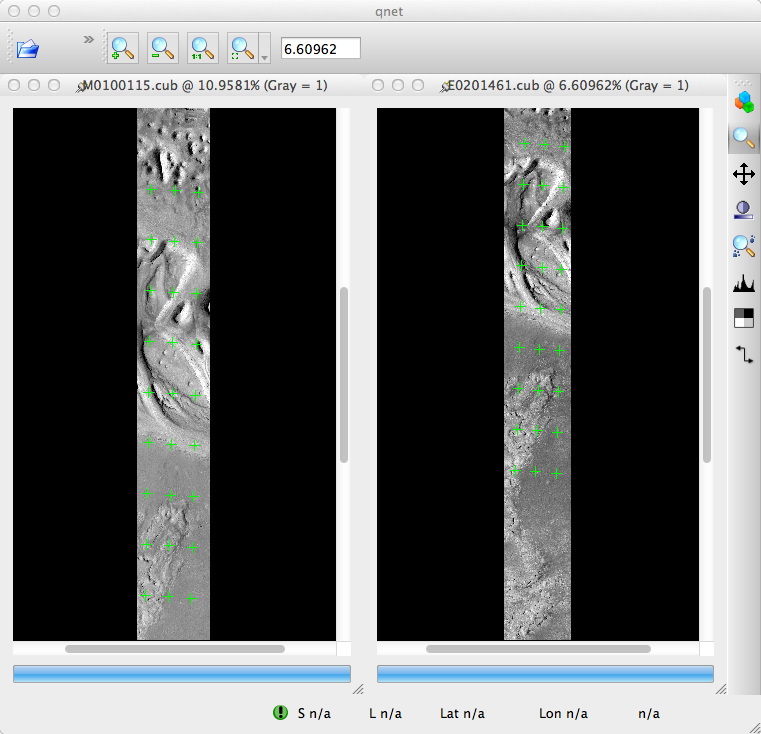
\includegraphics[width=5in]{images/qnet/Qnet_AfterAutoseed.png}
  \caption{A visualization of the features layed out by
    \texttt{autoseed} in \texttt{qnet}. Note that the marks do not
    cover the same features between images. This is due to the poor
    initial spice data for MOC imagery.}
  \label{fig:after_autoseed}
\end{figure}

\begin{verbatim}
  ISIS 3> autoseed fromlist=cube.lis overlaplist=overlap.lis    \
            onet=control.net deffile=autoseed.def networkid=moc \
            pointid=???? description=hrad_vallis
\end{verbatim}

The next step is to perform auto registration of these features
between the two images using \texttt{pointreg}. This program also
requires a settings file that describes how to do the automatic
search. Copy the text box below into a \textit{autoRegTemplate.def}
file.

\begin{verbatim}
   Object = AutoRegistration
    Group = Algorithm
      Name         = MaximumCorrelation
      Tolerance    = 0.7
    EndGroup

    Group = PatternChip
      Samples = 21
      Lines   = 21
      MinimumZScore = 1.5
      ValidPercent = 80
    EndGroup

    Group = SearchChip
      Samples = 75
      Lines   = 1000
    EndGroup
  EndObject
\end{verbatim}

The search chip defines the search range for which \texttt{pointreg}
will look for matching imagery. The pattern chip is simply the kernel
size of the matching template. The search range is specific for this
image pair. The control network result after \texttt{autoseed} had a
large vertical offset in the ball park of 500 px. The large
misalignment dictated the need for the large search in the lines
direction. Use \texttt{qnet} to get an idea for what the pixel shifts
look like in your stereo pair to help you decide on a search range. In
this example, only one measurement failed to match automatically. Here
are the arguments to use in this example of \texttt{pointreg}.

\begin{verbatim}
  ISIS 3> pointreg fromlist=cube.lis cnet=control.net             \
             onet=control_pointreg.net deffile=autoRegTemplate.def
\end{verbatim}

The third step is to manually edit the control and verify the
measurements in \texttt{qnet}. Type \texttt{qnet} in the terminal and
then open \textit{cube.lis} and lastly
\textit{control\_pointreg.net}. From the Control Network Navigator
window, click on the first point listed as \textit{0001}. That opens a
third window called the Qnet Tool. That window will allow you to play
a flip animation that shows alignment of the feature between the two
images. Correcting a measurement is performed by left clicking in the
right image, then clicking \textit{Save Measure}, and finally
finishing by clicking \textit{Save Point}.

In this tutorial, measurement \textit{0025} ended up being
incorrect. Your number may vary if you used different settings than
the above or if MOC spice data has improved since this writing. When
finished, go back to the main Qnet window. Save the final control
network as \textit{control\_qnet.net} by clicking on \textit{File},
and then \textit{Save As}.

\begin{figure}[ht]
  \centering
  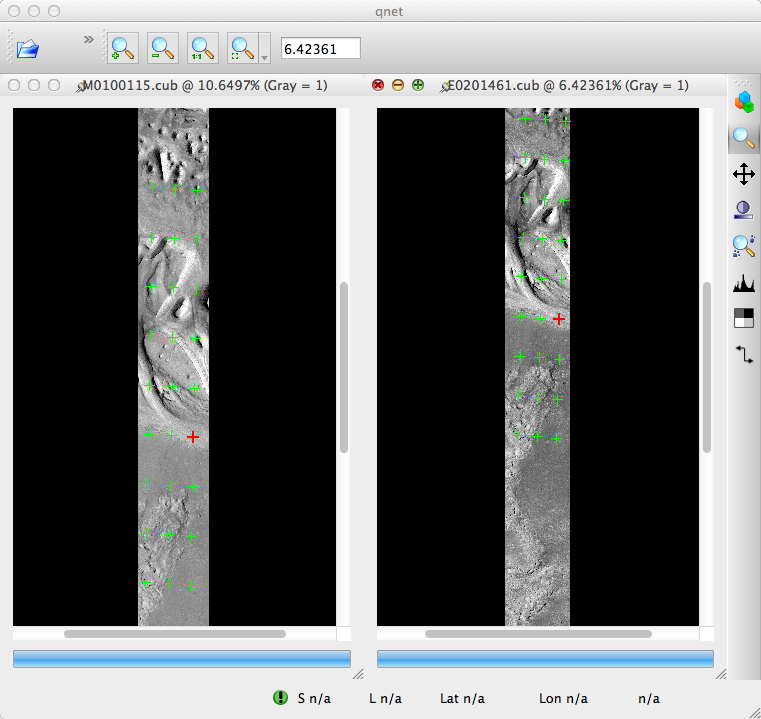
\includegraphics[width=5in]{images/qnet/Qnet_AfterQnetManual.png}
  \caption{A visualization of the features after manual editing in
    \texttt{qnet}. Note that the marks now appear in the same location
    between images.}
  \label{fig:after_autoseed}
\end{figure}

Once the control network is finished, it is finally time to start
bundle adjustment. Here's what the call to \texttt{jigsaw} looks like:

\begin{verbatim}
  ISIS 3> jigsaw fromlist=cube.lis update=yes twist=no radius=yes \
             cnet=control_qnet.net onet=control_ba.net
\end{verbatim}

The update option defines that we would like to update the camera
pointing, if our bundle adjustment converges. The \textit{twist=no}
says to not solve for the camera rotation about the camera bore. That
property is usually very well known as it is critical for integrating
an image with a line-scan camera. The \textit{radius=yes} means that
the radius of the 3D features can be solved for. Using no will force
the points to use height values from another source, usually LOLA or
MOLA.

The above command will spew out a bunch of diagnostic information from
every iteration of the optimization algorithm. The most important
feature to look at is the \textit{sigma0} value. It represents the mean of
pixel errors in the control network. In our run, the initial error was
1065 px and the final solution had an error of 1.1 px.

Producing a DEM using the newly created camera corrections is the same
as covered in the Tutorial on page \pageref{ch:tutorial}. When using
\texttt{jigsaw}, it modifies a copy of the spice data that is stored
internally to the cube file. Thus when we want to create a DEM using
the correct camera geometry, no extra information needs to be given to
\texttt{stereo} since it is already contained in the file. In the
event a mistake has been made, \texttt{spiceinit} will overwrite the
spice data inside a cube file and provide the original uncorrected
camera pointings.

\begin{verbatim}
  ISIS 3> stereo E0201461.cub M0100115.cub bundled/bundled
\end{verbatim}

%% \subsection{Processing with Ground Control Points}

%% Ground control point files describe a single point in the world
%% that is seen by 1 or more cameras. How they are measured in the
%% first place is up to the user. We use a manual process of comparing
%% each image to a respected map projected image and then recording
%% the latitude, longitude, and altitude of the point(s). The maps to
%% register against can be anything, but it is recommended to register
%% against a product with a high amount of cartographic stability and
%% accuracy.  For terrestrial work, we would use a \ac{USGS} product
%% that can provide imagery that is registered to LIDAR height
%% measurements.

%% Unlike match files, ground control points must specifically be given
%% to \texttt{isis\_adjust} from the command line, but in no particular
%% order. Ground control point files are written with the extension
%% \texttt{.gcp}. Below is an example of a ground control point file that
%% was created to control a series of Apollo Metric Camera images from
%% several Apollo 15 orbits.

%% \begin{verbatim}
%%     -52.8452 27.2561 1735999 300 300 500
%%     sub4-AS15-M-2086.cub     210.9   3565.0
%%     sub4-AS15-M-2087.cub     1476.9  3579.0
%%     sub4-AS15-M-2088.cub     2798.9  3586.8
%%     sub4-AS15-M-2089.cub     4133.5  3588.6
%%     sub4-AS15-M-2344.cub     906.9   3874.8
%%     sub4-AS15-M-2345.cub     2204.2  3913.9
%%     sub4-AS15-M-2482.cub     939.8   4348.0
%%     sub4-AS15-M-2483.cub     2282.0  4340.7
%%     sub4-AS15-M-2484.cub     3642.1  4330.9
%% \end{verbatim}

%% The first line of a \texttt{.gcp} file is like a header line and
%% is different from the remaining lines.  The first line defines the
%% world location of the ground control point, and the rest of the
%% lines define the image locations of the ground control points. Here
%% are what the columns mean for the first line.

%% \begin{myindentpar}{2cm}
%% \begin{description}
%%   \item[Column 1:] Longitude in degrees
%%   \item[Column 2:] Latitude in degrees
%%   \item[Column 3:] Radius in meters
%%   \item[Column 4:] Sigma (or uncertainty) in meters for Local X axis
%%   \item[Column 5:] Sigma (or uncertainty) in meters for Local Y axis
%%   \item[Column 6:] Sigma (or uncertainty) in meters for Local Z axis
%% \end{description}
%% \end{myindentpar}

%% The other lines describe where this \ac{GCP} is found in each image:

%% \begin{myindentpar}{2cm}
%% \begin{description}
%%   \item[Column 1:] Image name
%%   \item[Column 2:] Sample (X) image measurement
%%   \item[Column 3:] Line (Y) image measurement
%% \end{description}
%% \end{myindentpar}

%% Make a {\tt .gcp} file for every ground control point, then be sure
%% to feed them as an input to {\tt isis\_adjust}. Remember that you
%% can scale the sigma of all ground control points by using the {\tt
%% -\/-gcp-scalar} flag. This can save time by allowing you to make
%% adjustments without needing to edit all of the files individually.


\end{document}
